\chapter{Proyecto}
\label{cap:proyecto}

\section{Objetivos}
\label{sec:objetivos}

\subsection{Objetivo general}
Desarrollar una plataforma web basada en una arquitectura de microservicios mediante la integración de módulos de gestión documental y un motor de procesamiento de lenguaje natural para sistematizar el flujo operativo de recepción, clasificación y seguimiento de quejas de la DDP.

\subsection{Objetivos específicos}
\begin{itemize}
    \item \textbf{Analizar} el marco normativo de la Defensoría de los Derechos Politécnicos y sus manuales de procedimientos para definir las reglas de negocio que permitan la transición de la gestión analógica a un flujo de trabajo digitalizado.

    \item \textbf{Diseñar} la arquitectura del sistema basada en microservicios, asegurando la integridad de los datos y una experiencia de usuario (UX) accesible mediante:
    \begin{itemize}
        \item \textit{Arquitectura:} establecer un diseño modular que soporte la alta demanda de la comunidad politécnica y garantice la seguridad de la información sensible.
        \item \textit{Base de datos:} estructurar un esquema centralizado que elimine la duplicidad de registros y permita la trazabilidad total del expediente.
        \item \textit{UI/UX:} proyectar una interfaz intuitiva para el quejoso y un panel de gestión eficiente para el cuerpo técnico jurídico.
    \end{itemize}

    \item \textbf{Implementar} un módulo mediante técnicas de Procesamiento de Lenguaje Natural (PLN) para asistir en la clasificación preliminar de las quejas y determinar su competencia institucional.

    \item \textbf{Desarrollar} los componentes centrales de la plataforma web, garantizando la operatividad de las siguientes funciones:
    \begin{itemize}
        \item \textit{Gestión de expedientes:} digitalización del ciclo de vida de la queja (recepción, investigación y resolución) para optimizar el tiempo efectivo del personal jurídico.
        \item \textit{Seguimiento:} establecer un sistema de consulta para el quejoso que brinde transparencia sobre el estatus de su trámite.
        \item \textit{Gestión por roles:} implementar controles de acceso estrictos basados en las facultades normativas de cada actor dentro de la Defensoría.
    \end{itemize}
\end{itemize}

\section{Metodología}
\label{sec:metodologia}
Para el desarrollo del Trabajo Terminal se planteó inicialmente una metodología híbrida basada en Scrum-ban, con el fin de organizar en ciclos iterativos las tareas de desarrollo de software, diseño de interfaces y construcción de módulos funcionales. Conforme avanzó el proyecto, este esquema mostró limitaciones que afectaron la continuidad de los ciclos planteados, por lo que se sustituyó por un modelo incremental con prototipado evolutivo. En este apartado se exponen las razones del cambio, el enfoque adoptado y los incrementos en los que se organizó el desarrollo.

\subsection{Justificación del cambio de metodología}
Scrum-ban supone que el equipo cuenta con retroalimentación frecuente del cliente para priorizar, revisar y aceptar el trabajo de cada ciclo. En este proyecto, la Defensoría de los Derechos Politécnicos era la fuente de la retroalimentación operativa, de la validación funcional y de la definición de los requerimientos institucionales. Sin embargo, durante diversas etapas del proyecto existieron periodos prolongados sin disponibilidad para reuniones, revisión de avances o validación de cambios, lo que provocó modificaciones en las prioridades, en los requerimientos y en los tiempos de desarrollo.

Esta situación afectó la estabilidad del tablero Kanban y la planeación de los \textit{sprints}, ya que varias funcionalidades dependían de una validación institucional para darse por terminadas. En consecuencia, los ciclos no podían cerrarse en los tiempos previstos y el tablero dejó de reflejar el avance real del proyecto. Por ello, se determinó que Scrum-ban no representaba adecuadamente la dinámica del proyecto ni la forma en que evolucionaban sus requerimientos.

A lo anterior se suma que el proyecto no se limitó al desarrollo de software: involucró análisis normativo, modelado del procedimiento institucional, diseño arquitectónico, integración de componentes de inteligencia artificial y gestión documental. Estas actividades requieren periodos de investigación cuya duración es difícil de ajustar a ciclos de duración fija.

\subsection{Enfoque metodológico}
Se adoptó un modelo de desarrollo incremental con prototipado evolutivo \cite{pressman2014, sommerville2016}. En el desarrollo incremental, el sistema se construye por partes funcionales que se agregan sucesivamente a una base ya operativa; en el prototipado evolutivo, cada versión se presenta al cliente, se ajusta con sus observaciones y se conserva como base de la siguiente, en lugar de desecharse.

La principal razón de su elección es que permite desacoplar el avance técnico de la disponibilidad inmediata de validación institucional. Cuando la DDP no podía revisar un avance, el equipo continuaba con la arquitectura, el modelo de datos, las interfaces o los componentes de inteligencia artificial del siguiente incremento, y las observaciones recibidas posteriormente se incorporaban como ajustes al prototipo existente. De esta manera fue posible mantener la continuidad del desarrollo aun durante los periodos sin retroalimentación. Además, a diferencia de un enfoque ágil centrado únicamente en ciclos cortos de entrega, este modelo permitió trabajar de forma simultánea en actividades de distinta naturaleza: investigación normativa, diseño de la arquitectura distribuida, modelado de la base de datos, desarrollo del \textit{backend} y del \textit{frontend} e integración de inteligencia artificial.

Cada incremento siguió el mismo ciclo de trabajo:

\begin{enumerate}
    \item \textbf{Análisis:} identificación de las actividades, reglas de negocio y requerimientos del área correspondiente, a partir de los manuales institucionales y de las reuniones con el personal de la Defensoría.
    \item \textbf{Diseño:} definición de los casos de uso, los prototipos de interfaz, los cambios al modelo de datos y los servicios necesarios.
    \item \textbf{Construcción:} desarrollo de los microservicios y de las interfaces web del incremento.
    \item \textbf{Verificación:} pruebas del incremento y de su integración con los componentes ya construidos.
    \item \textbf{Revisión:} presentación del prototipo a la DDP cuando existió disponibilidad, e incorporación de sus observaciones en el mismo incremento o en uno posterior.
\end{enumerate}

\subsection{Incrementos del desarrollo}
El desarrollo se organizó en los siguientes incrementos. Aunque se presentan en orden, varios de ellos se trabajaron de forma parcialmente simultánea, precisamente para aprovechar los periodos sin retroalimentación institucional.

\begin{enumerate}
    \item \textbf{Análisis del procedimiento institucional:} revisión del marco normativo y de los manuales de la Defensoría, reuniones con su personal y elaboración del diagrama BPMN del proceso de atención de quejas.
    \item \textbf{Arquitectura base:} definición de los microservicios, del esquema de la base de datos, del mecanismo de autenticación y del despliegue en contenedores.
    \item \textbf{Portal del quejoso:} presentación de quejas con evidencias, consulta por folio, cuentas de seguimiento y notificaciones.
    \item \textbf{Recepción y administración:} panel de revisión para validar, rechazar y turnar quejas, registro de quejas en papel y consola de administración de cuentas, catálogos, plantillas y respaldos.
    \item \textbf{Primer Contacto y Subdefensoría:} análisis de los expedientes, citas, dictámenes y remisiones, así como la investigación con control de plazos y la elaboración de acuerdos.
    \item \textbf{Componentes de inteligencia artificial:} búsqueda de antecedentes y generación de resúmenes, integrados al módulo de Primer Contacto.
    \item \textbf{Supervisión de la Defensora:} panel de indicadores, seguimiento de las quejas por etapa y por unidad, y carga de trabajo del personal.
    \item \textbf{Pruebas y cierre:} verificación de la plataforma conforme a sus requerimientos funcionales y no funcionales, y corrección de los defectos encontrados.
\end{enumerate}

\section{Propuesta}
\label{sec:propuesta_proyecto}

\subsection{Qué se hará}
El Trabajo Terminal 2026-B009 propone el desarrollo de una plataforma web para la gestión de quejas de la Defensoría de los Derechos Politécnicos (DDP) del Instituto Politécnico Nacional. La plataforma abarcará los procesos de recepción, registro, revisión, atención y seguimiento de quejas mediante la administración de expedientes digitales, de modo que cada área de la Defensoría trabaje sobre la misma información y con los permisos que corresponden a su función.

El desarrollo utilizará una arquitectura basada en microservicios, con aplicaciones web independientes para cada perfil de usuario, e incorporará mecanismos de autenticación, autorización y control de acceso para proteger la información administrada. Como apoyo a la revisión de las quejas, se integrarán dos componentes de inteligencia artificial que funcionarán como herramientas de apoyo para el personal, sin sustituir su criterio ni las decisiones institucionales.

\subsection{Qué incluye la propuesta}
La propuesta contempla los siguientes componentes:

\begin{itemize}
    \item \textbf{Portal del quejoso:} registro de quejas con documentos y evidencias, con o sin cuenta; consulta del estado de la queja mediante folio; notificaciones y respuesta a acuerdos de conciliación.
    \item \textbf{Panel de Recepción:} validación, rechazo y turnado de quejas; registro de quejas recibidas en papel e historial de trámites.
    \item \textbf{Módulo de Primer Contacto:} análisis de expedientes, agenda de citas, oficios, dictamen de competencia y remisión a otras instancias.
    \item \textbf{Módulo de Subdefensoría:} investigación de los expedientes procedentes, solicitudes de información con control de plazos y acuerdos de conciliación y de conclusión.
    \item \textbf{Panel de la Defensora:} supervisión de las quejas y del personal, y administración de cuentas, catálogos, plantillas, respaldos y bitácora.
    \item \textbf{Componentes de inteligencia artificial:} un modelo de búsqueda de antecedentes y detección de posibles duplicidades mediante similitud semántica, y un modelo de generación de resúmenes narrativos que facilite la revisión de las quejas.
\end{itemize}

\subsection{Exclusiones}
La plataforma está orientada a su utilización mediante navegadores web, por lo que no contempla el desarrollo de una aplicación móvil nativa ni la integración con sistemas externos al alcance definido. Tampoco contempla la emisión automatizada de resoluciones o dictámenes jurídicos, ya que estas actividades corresponden exclusivamente al personal autorizado de la Defensoría.

\section{Riesgos y supuestos}
\label{sec:riesgos_supuestos}
\label{sec:limitaciones}
El desarrollo, la implementación y la evaluación del Trabajo Terminal están sujetos a condiciones académicas, tecnológicas e institucionales que pueden influir en el alcance y el funcionamiento de la plataforma. En este apartado se identifican los riesgos del proyecto, con la acción adoptada para mitigar cada uno, y los supuestos sobre los que se planteó la propuesta.

\subsection{Riesgos}

\rowcolors{2}{rowblue}{white}
\small
\renewcommand{\arraystretch}{1.25}
\setlength{\tabcolsep}{4pt}
\begin{longtable}{|L{3.0cm}|L{6.4cm}|L{6.2cm}|}
	\hiderowcolors\caption{Riesgos del proyecto y acciones de mitigación}
	\label{tab:riesgos} \\ \showrowcolors
	\hline
	\rowcolor{headerblue}
	\headercell{Riesgo} & \headercell{Descripción} & \headercell{Mitigación} \\
	\hline
	\endfirsthead
	\hline
	\rowcolor{headerblue}
	\headercell{Riesgo} & \headercell{Descripción} & \headercell{Mitigación} \\
	\hline
	\endhead
	Tiempo de desarrollo & Al tratarse de un proyecto académico con un periodo de ejecución definido, la implementación, integración y validación de los módulos están sujetas al calendario de entregas; algunas funcionalidades podrían quedar incompletas. & Desarrollo incremental que prioriza el flujo principal de atención de quejas y registro explícito del estado de avance de cada componente. \\ \hline
	Disponibilidad de la DDP para validar & Los periodos sin disponibilidad del personal para reuniones o revisiones pueden retrasar la validación de requerimientos y cambios. & Prototipado evolutivo: el desarrollo continúa con otros incrementos y las observaciones se incorporan después al prototipo. \\ \hline
	Disponibilidad de datos & El desarrollo y la evaluación de los modelos de inteligencia artificial dependen de expedientes históricos, cuyo acceso está restringido por tratarse de información sensible. & Uso de conjuntos de datos sintéticos, cuyos resultados se interpretan como preliminares; la validación con expedientes reales queda como trabajo futuro. \\ \hline
	Precisión de los modelos & La búsqueda de antecedentes puede señalar casos que no son duplicidades reales u omitir coincidencias relevantes; el modelo de resúmenes puede presentar omisiones, interpretaciones incorrectas o información no sustentada en el texto original. & Los resultados se presentan como sugerencias o borradores que siempre requieren revisión del personal. \\ \hline
	Infraestructura tecnológica & El funcionamiento de la plataforma y de los modelos depende de la capacidad de procesamiento, memoria y almacenamiento disponible, lo que puede limitar el rendimiento y la ejecución simultánea de servicios. & Los servicios de inteligencia artificial se ejecutan por separado, de modo que su falla o saturación no detiene la operación del resto de la plataforma. \\ \hline
	Protección de datos personales & Los expedientes contienen datos personales y situaciones sensibles cuya exposición tendría consecuencias para las personas involucradas. & Cifrado de las comunicaciones, control de acceso por rol y registro de las acciones administrativas en bitácora. \\ \hline
\end{longtable}
\normalsize
\setlength{\tabcolsep}{6pt}
\renewcommand{\arraystretch}{1}

\subsection{Supuestos}
La propuesta se planteó considerando los siguientes supuestos:

\begin{itemize}
    \item El procedimiento descrito en los manuales de la Defensoría permanece vigente durante el desarrollo, por lo que las reglas de negocio derivadas de ellos siguen siendo válidas.
    \item El personal de la Defensoría participa en reuniones de revisión y validación en los momentos clave del proyecto, aunque no sea de manera continua.
    \item Los usuarios acceden a la plataforma mediante un navegador web actualizado y con conexión a Internet.
    \item Se dispone de servidores para desplegar los contenedores de la plataforma y de un servicio de correo electrónico para el envío de notificaciones.
    \item El tratamiento de expedientes y datos personales se ajusta a las disposiciones institucionales y a la normativa aplicable en materia de protección de datos.
    \item El personal autorizado revisa los resultados de los componentes de inteligencia artificial antes de utilizarlos, ya que estos no sustituyen la revisión, interpretación ni las decisiones jurídicas de la Defensoría.
\end{itemize}


	\section{Actores del sistema}
	\label{sec:actores}
	El análisis distingue a la persona que presenta la queja y a los perfiles institucionales
	que participan en su recepción, análisis, gestión y seguimiento. La organización por roles
	justifica aplicaciones web diferenciadas y políticas de autorización en los servicios: la
	separación de interfaces mejora la adaptación al trabajo de cada área, aunque no sustituye
	la validación de permisos en el servidor.
	
	\begin{itemize}
		\item \textbf{Quejoso.} Cualquier integrante de la comunidad politécnica ---estudiante,
		personal académico o administrativo--- que presenta una queja o le da seguimiento. Es el
		único actor externo y el único que puede operar sin credenciales previas.
	
		\item \textbf{Personal de recepción.} Personal de la Defensoría encargado de recibir,
		validar y canalizar las quejas que llegan por el portal público o en papel.
	
		\item \textbf{Analista de primer contacto.} Consulta expedientes, revisa antecedentes
		relacionados y utiliza borradores de resumen como apoyo al análisis de quejas.
		\item \textbf{Subdefensoría.} Gestiona las actuaciones y el seguimiento que corresponden
		a su área conforme a los permisos asignados.
		\item \textbf{Defensora.} Titular de la Defensoría. Participa en las etapas de decisión y
		resolución del expediente, sin que las herramientas de inteligencia artificial sustituyan sus
		atribuciones; supervisa la operación desde su panel y administra la plataforma: cuentas del
		personal, catálogos, plantillas, respaldos y bitácora de seguridad.
	\end{itemize}
	
	La Tabla~\ref{tab:actores_roles} presenta los perfiles, su rol en el sistema y sus
	responsabilidades generales.

	\rowcolors{2}{rowblue}{white}
	\small
	\renewcommand{\arraystretch}{1.25}
	\setlength{\tabcolsep}{4pt}
	\begin{longtable}{|L{3.8cm}|L{4.8cm}|L{7.0cm}|}
		\hiderowcolors\caption{Actores y roles del sistema}
		\label{tab:actores_roles} \\ \showrowcolors
		\hline
		\rowcolor{headerblue}
		\headercell{Actor} & \headercell{Rol en el sistema} & \headercell{Responsabilidad} \\
		\hline
		\endfirsthead
		\hline
		\rowcolor{headerblue}
		\headercell{Actor} & \headercell{Rol en el sistema} & \headercell{Responsabilidad} \\
		\hline
		\endhead
		Quejoso & ---\ (usuario externo) & Presentar quejas y darles seguimiento \\ \hline
		Personal de recepción & \texttt{RECEPCIONISTA} & Recibir, validar, rechazar y turnar quejas \\ \hline
		Analista de primer contacto & \texttt{ANALISTA\_\allowbreak PRIMER\_\allowbreak CONTACTO} & Análisis de expedientes y consulta de herramientas de inteligencia artificial \\ \hline
		Subdefensor & \texttt{SUBDEFENSOR} & Gestión y seguimiento de actuaciones de su área \\ \hline
		Defensora & \texttt{DEFENSOR} & Supervisión, resolución y cierre del expediente; administración de cuentas, catálogos, plantillas, respaldos y bitácora \\ \hline
	\end{longtable}
	\normalsize
	\setlength{\tabcolsep}{6pt}
	\renewcommand{\arraystretch}{1}

	La Figura~\ref{fig:organigrama} muestra la estructura de la Defensoría y el rol que corresponde a cada área en la plataforma. La Defensoría cuenta con dos subdefensorías ---Atención a los Alumnos y Egresados, y Atención a Personal---, ambas con el rol \texttt{SUBDEFENSOR}.

	\begin{figure}[H]
		\centering
		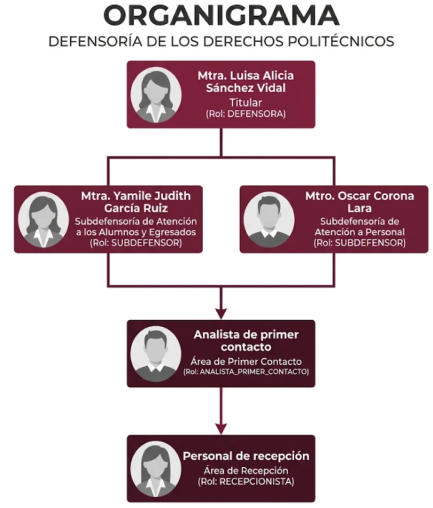
\includegraphics[width=0.6\textwidth]{images/organigrama_ddp.png}
		\caption{Organigrama de la Defensoría de los Derechos Politécnicos y roles en la plataforma}
		\label{fig:organigrama}
	\end{figure}

	Los módulos de Primer Contacto y Subdefensoría forman parte del flujo de trabajo de la
	plataforma. Sus permisos y servicios deben documentarse de manera coherente con la matriz
	de autorización y los casos de uso. Las actividades de resolución corresponden al personal
	institucional autorizado y no se automatizan mediante inteligencia artificial.
	
	\section{Especificación de requerimientos}
	\label{sec:requerimientos}
	El levantamiento de requerimientos combinó la revisión de documentación institucional
	de la Defensoría con reuniones de trabajo para precisar actividades, responsabilidades
	y necesidades de los distintos perfiles. El equipo sostuvo una serie de reuniones con el personal
	de la institución que evolucionaron de forma iterativa: cada sesión aclaró aspectos que la
	anterior había dejado abiertos, y cada avance técnico intermedio se convirtió en insumo de la
	siguiente reunión.
	
	La primera sesión tuvo como objetivo comprender el contexto operativo e identificar las áreas
	que intervienen en la gestión de una queja. Con ese contexto el equipo elaboró un diagrama de
	proceso en notación BPMN a partir de los documentos oficiales, que se presentó en una segunda
	sesión como base de discusión. La revisión permitió aclarar el alcance y la secuencia de distintas actividades,
	incorporar observaciones del personal y ajustar el diagrama para representar el flujo
	de atención acordado para la plataforma. Validado ese diagrama, se establecieron
	sesiones por área para traducir las actividades de cada rol en casos de uso y vistas concretas,
	con sesiones de revisión intermedias para confirmar que los artefactos reflejaran lo acordado.
	
	El resultado acumulado se organizó en tres categorías ---requerimientos funcionales, no
	funcionales y reglas de negocio--- y se estructuró por actor, de modo que cada requerimiento
	tiene un dueño identificable. La nomenclatura empleada codifica el actor en el identificador:
	\texttt{RF-Q} para los requerimientos funcionales del quejoso, \texttt{RF-R} para los del
	personal de recepción, \texttt{RF-PC} para los de Primer Contacto, \texttt{RF-SD} para los de
	Subdefensoría y \texttt{RF-A} para los de la Defensora, y de forma análoga
	\texttt{RNF-} y \texttt{RN-} para los no funcionales y las reglas de negocio. Esta convención permite rastrear cada elemento hasta su origen.
	
	\subsection{Requerimientos funcionales del quejoso}
	Los requerimientos del quejoso se agrupan en cinco bloques: operación sin cuenta, gestión de la
	cuenta, gestión de las quejas propias, seguimiento y servicios de apoyo. El primer bloque es el
	más determinante para el diseño, porque exige que el sistema acepte quejas de personas que no
	tienen ---ni necesariamente quieren tener--- una cuenta, lo que obliga a un punto de acceso
	público sin autenticación y a un mecanismo de identificación posterior basado en el folio.
	
	\small
	\renewcommand{\arraystretch}{1.2}
	\setlength{\tabcolsep}{4pt}
	
	\begin{longtable}{|L{1.7cm}|L{4.0cm}|L{9.9cm}|}
		\hiderowcolors\caption{Requerimientos funcionales del actor Quejoso}
		\label{tab:rf_quejoso} \\ \showrowcolors
		\hline
		\rowcolor{headerblue}
		\headercell{ID} & \headercell{Requerimiento} & \headercell{Descripción} \\
		\hline
		\endfirsthead
	
		\hline
		\rowcolor{headerblue}
		\headercell{ID} & \headercell{Requerimiento} & \headercell{Descripción} \\
		\hline
		\endhead
	
		RF-Q01 & Consultar una queja sin cuenta & Dado un folio y el correo con que se presentó,
		mostrar el detalle de la queja: motivo, descripción, estatus y fecha. \\ \hline
	
		RF-Q02 & Registrar una queja sin cuenta & Capturar la identidad completa del quejoso,
		unidad académica, fecha de los hechos, datos del denunciado, descripción libre y varios
		archivos de evidencia en una sola petición; generar un folio de seguimiento. \\ \hline
	
		RF-Q03 & Capturar datos del tutor & Si la fecha de nacimiento indica que el quejoso es menor
		de edad, exigir los datos de un tutor o adulto responsable antes de permitir el envío.
		\\ \hline
	
		RF-Q04 & Activar una cuenta de seguimiento & A partir de un folio y correo ya registrados en
		una queja existente, definir una contraseña y activar la cuenta. \\ \hline
	
		RF-Q05 & Iniciar sesión & Autenticarse con correo institucional y contraseña, obteniendo un
		token de sesión con vigencia limitada. \\ \hline
	
		RF-Q06 & Recuperar la contraseña & Restablecer la contraseña mediante un código de
		verificación de seis dígitos enviado por correo electrónico. \\ \hline
	
		RF-Q07 & Consultar un resumen de actividad & Mostrar al entrar al panel el conteo de quejas
		propias agrupadas por estatus. \\ \hline
	
		RF-Q08 & Listar y consultar las quejas propias & Listar las quejas del usuario con filtros
		por estatus y texto, y mostrar el detalle completo de cada una con su línea de tiempo de
		estatus. \\ \hline
	
		RF-Q09 & Editar una queja propia & Modificar descripción, unidad académica, fecha de hechos
		y datos del denunciado, únicamente mientras la queja no haya iniciado su validación.
		\\ \hline
	
		RF-Q10 & Registrar una queja autenticado & Presentar una queja nueva desde el panel sin
		volver a capturar la identidad, que se toma del token de sesión. \\ \hline
	
		RF-Q11 & Consultar las evidencias propias & Previsualizar y descargar los archivos adjuntos
		a una queja propia. \\ \hline
	
		RF-Q12 & Responder acuerdos de conciliación & Consultar los acuerdos propuestos por la
		Defensoría y aceptarlos o rechazarlos, con comentario opcional. \\ \hline
	
		RF-Q13 & Consultar el centro de notificaciones & Consultar un historial persistente de
		avisos con contador de no leídas y marcado individual como leída. \\ \hline
	
		RF-Q14 & Consultar y editar el perfil & Editar correo personal, teléfono, unidad académica y
		domicilio; consultar en modo de solo lectura el nombre, el correo institucional y la boleta o
		número de empleado. \\ \hline
	
		RF-Q15 & Consultar el catálogo institucional & Seleccionar la dependencia o unidad académica
		involucrada desde el catálogo del Instituto, en lugar de capturarla como texto libre.
		\\ \hline
	
		RF-Q16 & Consultar preguntas frecuentes & Consultar sin sesión un menú fijo de preguntas y
		respuestas sobre la Defensoría y el proceso de queja. \\ \hline
	
		RF-Q17 & Recibir avisos por correo & Recibir confirmación de creación de cuenta, confirmación
		de restablecimiento de contraseña y, en el caso de menores de edad, aviso al tutor.
		\\ \hline
	\end{longtable}
	
	\normalsize
	
	\subsection{Requerimientos funcionales del personal de recepción}
	El diseño de este bloque partió de una restricción que el propio personal planteó en las
	sesiones de levantamiento: no todas las quejas llegan por el portal. Una parte del volumen
	ingresa en papel, y el sistema debía poder incorporarlas al mismo flujo digital sin obligar al
	quejoso a capturarlas de nuevo. De ahí el requerimiento de registro manual (RF-R08), que es la
	razón por la que el modelo de datos distingue el origen de cada queja.
	
	\small
	\renewcommand{\arraystretch}{1.2}
	
	\begin{longtable}{|L{1.7cm}|L{4.0cm}|L{9.9cm}|}
		\hiderowcolors\caption{Requerimientos funcionales del actor Personal de recepción}
		\label{tab:rf_recepcion} \\ \showrowcolors
		\hline
		\rowcolor{headerblue}
		\headercell{ID} & \headercell{Requerimiento} & \headercell{Descripción} \\
		\hline
		\endfirsthead
	
		\hline
		\rowcolor{headerblue}
		\headercell{ID} & \headercell{Requerimiento} & \headercell{Descripción} \\
		\hline
		\endhead
	
		RF-R01 & Iniciar sesión & Autenticarse con las credenciales de personal administrativo desde
		el panel de revisión. \\ \hline
	
		RF-R02 & Consultar la bandeja de entrada & Consultar la lista de quejas por trabajar, con
		contadores de pendientes, en proceso y turnadas en el día. \\ \hline
	
		RF-R03 & Consultar el detalle de una queja & Consultar el resumen completo del expediente y
		los documentos adjuntos, para su validación. \\ \hline
	
		RF-R04 & Buscar antecedentes & Consultar quejas anteriores potencialmente relacionadas,
		por hechos o personas involucradas, como apoyo para identificar antecedentes y posibles duplicidades. \\ \hline
	
		RF-R05 & Consultar los documentos adjuntos & Previsualizar y descargar las evidencias
		asociadas a una queja. \\ \hline
	
		RF-R06 & Rechazar una queja & Rechazar una queja por documentación incompleta, indicando
		motivos y observaciones, con notificación automática al quejoso. \\ \hline
	
		RF-R07 & Turnar una queja & Canalizar la queja a un área o dependencia y a un defensor o
		subdefensor específico, con comentarios, generando el folio oficial de turnado. \\ \hline
	
		RF-R08 & Registrar una queja recibida en papel & Dar de alta manualmente una queja física
		con la identidad del quejoso, dependencia, número de oficio, fecha de recepción, tipo de
		documento, descripción, ubicación física del expediente y un archivo digitalizado opcional.
		\\ \hline
	
		RF-R09 & Consultar el historial de trámites & Consultar los trámites ya procesados, con
		filtros por texto, estatus y fecha. \\ \hline
	
		RF-R10 & Exportar el historial & Exportar el historial filtrado a un archivo de hoja de
		cálculo. \\ \hline
	
		RF-R11 & Emitir un acuerdo de conciliación & Emitir un acuerdo dirigido al quejoso de una
		queja, con asunto y términos. \\ \hline
	
		RF-R12 & Consultar catálogos de apoyo & Consultar la lista de dependencias y la de personal
		disponible para turnado. \\ \hline
	
		RF-R13 & Cambiar la propia contraseña & Modificar la contraseña de la cuenta propia desde el
		panel. \\ \hline
	\end{longtable}
	
	\normalsize
	
	\subsection{Requerimientos funcionales de Primer Contacto}
	Primer Contacto es la etapa en la que se decide si la Defensoría es competente para conocer la
	queja. Recepción turna cada queja a un analista, y cada analista trabaja únicamente los
	expedientes que tiene asignados. La Tabla~\ref{tab:rf_pc} reúne sus requerimientos.

	\small
	\renewcommand{\arraystretch}{1.2}

	\begin{longtable}{|L{1.7cm}|L{4.0cm}|L{9.9cm}|}
		\hiderowcolors\caption{Requerimientos funcionales del actor Analista de Primer Contacto}
		\label{tab:rf_pc} \\ \showrowcolors
		\hline
		\rowcolor{headerblue}
		\headercell{ID} & \headercell{Requerimiento} & \headercell{Descripción} \\
		\hline
		\endfirsthead

		\hline
		\rowcolor{headerblue}
		\headercell{ID} & \headercell{Requerimiento} & \headercell{Descripción} \\
		\hline
		\endhead

		RF-PC01 & Recibir quejas turnadas & Crear el expediente de análisis cuando Recepción turna una
		queja, con el analista asignado, su prioridad, quejoso, narración y evidencias. \\ \hline

		RF-PC02 & Consultar la bandeja de análisis & Listar los expedientes asignados al analista con
		filtros por folio, prioridad y estatus, e indicadores, pendientes y citas del día en un tablero
		de inicio. \\ \hline

		RF-PC03 & Abrir un expediente & Iniciar el análisis al abrir el expediente y presentar la
		narración, los datos de la queja, del quejoso y de la persona señalada, las evidencias y el
		historial; impedir el acceso a expedientes asignados a otro analista. \\ \hline

		RF-PC04 & Gestionar la agenda de citas & Programar citas con el quejoso y con la persona
		señalada (comparecencia, revisión de documentos o seguimiento; presencial o virtual) en horario
		hábil, sin empalmes ni fines de semana; confirmarlas, reagendarlas o cancelarlas, y avisar a la
		persona citada con un enlace para responder. \\ \hline

		RF-PC05 & Elaborar oficios de análisis & Redactar oficios con asunto y contenido, numerados
		\texttt{DDP/PC/OF/año/id}, generarlos en PDF, y editarlos o eliminarlos solo por su autor.
		\\ \hline

		RF-PC06 & Registrar la versión de la persona señalada & Capturar la versión que la persona
		señalada rinde ante el analista, con su identificación, fecha de entrevista y evidencias,
		dejando constancia de quién la registró. \\ \hline

		RF-PC07 & Dictaminar la competencia & Declarar la queja procedente con justificación y
		observaciones, elegir al abogado responsable en Subdefensoría de una lista ordenada por carga
		de trabajo y turnar el expediente; permitir reenviarlo si Subdefensoría no lo recibió.
		\\ \hline

		RF-PC08 & Dictaminar la improcedencia y remitir & Declarar la queja improcedente con
		justificación y remitirla a la instancia competente (Abogado General, Órgano Interno de
		Control o instancias del Protocolo de Género): generar el oficio en PDF, enviarlo por correo
		a la instancia y avisar al quejoso. \\ \hline

		RF-PC09 & Proponer una conciliación & Registrar una propuesta de conciliación desde el
		expediente. \\ \hline

		RF-PC10 & Asignar la prioridad & Asignar al expediente una prioridad (baja, media, alta o
		urgente) mientras esté abierto o, ya dictaminado procedente, antes de que Subdefensoría lo
		reciba. \\ \hline
	\end{longtable}

	\normalsize

	\subsection{Requerimientos funcionales de Subdefensoría}
	La Subdefensoría investiga los expedientes procedentes. Cada abogado trabaja los expedientes que
	le asignó Primer Contacto, mientras que el titular de la Defensoría puede consultarlos todos.
	Sus requerimientos (Tabla~\ref{tab:rf_sd}) están dominados por los plazos que fija el Manual de
	Procedimientos de la DDP: diez días hábiles para que una unidad responda la primera solicitud de
	información y cinco para cada recordatorio \cite{ipn_manual_procedimientos_ddp}.

	\small
	\renewcommand{\arraystretch}{1.2}

	\begin{longtable}{|L{1.7cm}|L{4.0cm}|L{9.9cm}|}
		\hiderowcolors\caption{Requerimientos funcionales del actor Abogado de Subdefensoría}
		\label{tab:rf_sd} \\ \showrowcolors
		\hline
		\rowcolor{headerblue}
		\headercell{ID} & \headercell{Requerimiento} & \headercell{Descripción} \\
		\hline
		\endfirsthead

		\hline
		\rowcolor{headerblue}
		\headercell{ID} & \headercell{Requerimiento} & \headercell{Descripción} \\
		\hline
		\endhead

		RF-SD01 & Recibir el expediente & Crear el expediente de investigación, asignado al abogado
		elegido, cuando Primer Contacto dictamina la queja como procedente. \\ \hline

		RF-SD02 & Consultar el inicio y los pendientes & Mostrar indicadores, pendientes del día
		ordenados por urgencia, expedientes que vencen pronto y su distribución por etapa. \\ \hline

		RF-SD03 & Consultar los expedientes propios & Listar los expedientes por etapa (por abrir, por
		solicitar oficio, esperando respuesta de la unidad, por redactar acuerdo, esperando respuesta
		del quejoso, concluidos) con búsqueda, filtros por prioridad y plazo, barra de plazo, siguiente
		paso sugerido y exportación. \\ \hline

		RF-SD04 & Abrir un expediente & Iniciar la investigación y consultar, en modo de solo lectura,
		lo actuado en Primer Contacto: oficios, citas y dictamen. \\ \hline

		RF-SD05 & Solicitar información a la unidad & Seleccionar la unidad académica del catálogo
		institucional, redactar el oficio de solicitud de información y enviarlo por correo a su
		titular, con PDF y plazo de diez días hábiles. \\ \hline

		RF-SD06 & Enviar un recordatorio de urgencia & Enviar un recordatorio a la unidad que no
		respondió, con plazo de cinco días hábiles. \\ \hline

		RF-SD07 & Registrar la respuesta de la unidad & Registrar la respuesta de la unidad con su canal
		de recepción, resumen y archivo. \\ \hline

		RF-SD08 & Elaborar el acuerdo de conciliación & Elaborar el acuerdo de conciliación y enviarlo
		al quejoso, quien lo acepta o rechaza mediante un enlace. \\ \hline

		RF-SD09 & Elaborar el acuerdo de conclusión & Elaborar y enviar el acuerdo de conclusión y
		cerrar el expediente. \\ \hline

		RF-SD10 & Controlar los plazos & Mostrar el semáforo de plazos y las alertas de oficios
		vencidos o por vencer en tres días o menos. \\ \hline

		RF-SD11 & Asignar la prioridad & Cambiar la prioridad del expediente (baja, media, alta o
		urgente) y ordenar la bandeja de mayor a menor prioridad. \\ \hline
	\end{longtable}

	\normalsize

	\subsection{Requerimientos funcionales de la Defensora}
	Este bloque concentra las funciones que hacen operable la plataforma a largo plazo sin
	intervención del equipo de desarrollo. Su requerimiento más sensible es el de respaldo y
	restauración (RF-A06), porque incluye la única operación destructiva de todo el sistema y por
	ello recibe un tratamiento de seguridad diferenciado.
	
	\small
	\renewcommand{\arraystretch}{1.2}
	
	\begin{longtable}{|L{1.7cm}|L{4.0cm}|L{9.9cm}|}
		\hiderowcolors\caption{Requerimientos funcionales del actor Defensora}
		\label{tab:rf_admin} \\ \showrowcolors
		\hline
		\rowcolor{headerblue}
		\headercell{ID} & \headercell{Requerimiento} & \headercell{Descripción} \\
		\hline
		\endfirsthead
	
		\hline
		\rowcolor{headerblue}
		\headercell{ID} & \headercell{Requerimiento} & \headercell{Descripción} \\
		\hline
		\endhead
	
		RF-A01 & Iniciar sesión & Autenticarse como personal administrativo. \\ \hline
	
		RF-A02 & Consultar el tablero general & Consultar un resumen del estado del sistema al
		entrar a la consola. \\ \hline
	
		RF-A03 & Gestionar cuentas de personal & Listar, crear con contraseña temporal, editar,
		restablecer contraseña, dar de baja y reactivar cuentas de cualquiera de los cinco roles.
		\\ \hline
	
		RF-A04 & Administrar el catálogo institucional & Listar, crear y editar dependencias, e
		importar o actualizar el catálogo de forma masiva desde un archivo de hoja de cálculo.
		\\ \hline
	
		RF-A05 & Administrar plantillas de documentos & Listar plantillas, consultar los marcadores
		disponibles, previsualizar con datos de ejemplo y editar o publicar su contenido. \\ \hline
	
		RF-A06 & Gestionar respaldos de la base de datos & Listar los respaldos existentes, ejecutar
		un respaldo bajo demanda, descargar un respaldo y restaurar la base de datos a partir de uno
		de ellos. \\ \hline
	
		RF-A07 & Consultar la bitácora de acciones críticas & Consultar el registro de acciones
		administrativas con usuario, acción, dirección de origen y fecha. \\ \hline
	
		RF-A08 & Administrar el contenido de preguntas frecuentes & Listar, crear, editar y eliminar
		las preguntas del portal público. \\ \hline
	
		RF-A09 & Cambiar la propia contraseña & Modificar la contraseña de la cuenta propia desde la
		consola. \\ \hline
	\end{longtable}
	
	\normalsize
	\setlength{\tabcolsep}{6pt}
	\renewcommand{\arraystretch}{1}
	
	\subsection{Requerimientos no funcionales}
	Los requerimientos no funcionales expresan atributos de calidad y no funciones. Se agruparon en
	tres características: \textbf{funcionalidad}, que verifica que el sistema haga cumplir
	correctamente sus reglas e informe el resultado de cada operación; \textbf{robustez}, que
	verifica que el sistema mantenga su operación ante fallos de servicios auxiliares o entradas
	incorrectas; y \textbf{seguridad}, que verifica la protección de la información y el control de
	acceso. La Tabla~\ref{tab:rnf} los concentra.

	\rowcolors{2}{rowblue}{white}
	\small
	\renewcommand{\arraystretch}{1.2}
	\setlength{\tabcolsep}{4pt}
	\begin{longtable}{|L{1.8cm}|L{2.7cm}|L{11.1cm}|}
		\hiderowcolors\caption{Requerimientos no funcionales de la plataforma}
		\label{tab:rnf} \\ \showrowcolors
		\hline
		\rowcolor{headerblue}
		\headercell{ID} & \headercell{Característica} & \headercell{Atributo requerido} \\
		\hline
		\endfirsthead
		\hline
		\rowcolor{headerblue}
		\headercell{ID} & \headercell{Característica} & \headercell{Atributo requerido} \\
		\hline
		\endhead
		RNF-G01 & Funcionalidad & Las reglas de negocio deben validarse en el servidor y no solo en
		la interfaz; una operación no permitida se rechaza aunque se invoque directamente la interfaz
		de programación. \\ \hline
		RNF-Q07 & Funcionalidad & Toda operación debe producir retroalimentación visual inmediata de
		éxito, error o validación; no se admiten fallos silenciosos. \\ \hline
		RNF-Q04 & Robustez & Un fallo en el envío de un correo ---incluido el de rechazo de una
		queja--- o en el registro de una notificación nunca debe impedir que la operación principal se
		complete; el fallo se degrada a un registro en la bitácora del servidor. \\ \hline
		RNF-A04 & Robustez & La importación masiva del catálogo debe reportar un resumen de filas
		procesadas, creadas, actualizadas y con error, en lugar de fallar en bloque ante una fila mal
		formada. \\ \hline
		RNF-G02 & Robustez & Una falla o indisponibilidad de los servicios de inteligencia artificial
		no debe bloquear la recepción, el seguimiento ni las decisiones administrativas del
		expediente. \\ \hline
		RNF-Q02 & Seguridad & Todo el tráfico público debe viajar cifrado con TLS; tras el inicio de
		sesión, la autenticación se transmite como token en el encabezado de autorización y nunca como
		credenciales en claro. \\ \hline
		RNF-Q06 & Seguridad & La sesión del quejoso debe expirar en una hora; al expirar o ser
		rechazada, el cliente debe cerrar sesión de forma automática. \\ \hline
		RNF-R02 & Seguridad & El personal debe autenticarse en un único punto; ningún panel de
		personal implementa lógica de contraseñas propia. \\ \hline
		RNF-A01 & Seguridad & El primer acceso administrativo debe autoprovisionarse en el arranque
		inicial con una contraseña temporal registrada una sola vez en la bitácora del servidor; nunca
		incrustada en el cliente ni expuesta por la interfaz de programación. \\ \hline
		RNF-A03 & Seguridad & La restauración de la base de datos debe exigir una confirmación
		explícita en el cuerpo de la petición; no puede dispararse con una sola acción accidental. \\ \hline
		RNF-A06 & Seguridad & La generación, descarga y restauración de respaldos debe estar
		disponible únicamente para el rol de la Defensora (\texttt{DEFENSOR}). \\ \hline
	\end{longtable}
	\normalsize
	\setlength{\tabcolsep}{6pt}
	\renewcommand{\arraystretch}{1}

	\subsection{Reglas de negocio}
	Las reglas de negocio son las restricciones que el sistema debe hacer cumplir para que el
	procedimiento sea válido. A diferencia de los requerimientos funcionales, que describen lo que
	el sistema \emph{permite} hacer, las reglas describen lo que \emph{prohíbe} o \emph{obliga}. Su
	característica común en esta plataforma es que se validan en el servidor y no solo en la
	interfaz: ocultar un botón no es hacer cumplir una regla, y así se hace explícito en varias de
	las que siguen.
	
	\small
	\renewcommand{\arraystretch}{1.2}
	
	\begin{longtable}{|L{1.8cm}|L{2.7cm}|L{11.1cm}|}
		\hiderowcolors\caption{Reglas de negocio de la plataforma}
		\label{tab:reglas_negocio} \\ \showrowcolors
		\hline
		\rowcolor{headerblue}
		\headercell{ID} & \headercell{Temática} & \headercell{Regla} \\
		\hline
		\endfirsthead
	
		\hline
		\rowcolor{headerblue}
		\headercell{ID} & \headercell{Temática} & \headercell{Regla} \\
		\hline
		\endhead
	
		RN-Q01 & Menores de edad & Una queja de una persona menor de 18 años requiere datos de tutor
		o adulto responsable capturados y confirmados antes de poder enviarse. \\ \hline
	
		RN-Q02 & Menores de edad & Una persona menor de 14 años no puede autorregistrarse ni
		gestionar la queja por sí misma; la interfaz indica de forma explícita que debe ser el tutor
		quien complete el formulario a su nombre. \\ \hline
	
	
		RN-Q04 & Activación & Una cuenta de quejoso solo puede activarse si existe al menos una queja
		previa con ese folio \emph{y} ese correo; el par folio-correo es la llave de activación.
		\\ \hline
	
	
		RN-Q06 & Contraseñas & La contraseña debe tener al menos ocho caracteres, una mayúscula y un
		dígito, tanto en la activación de cuenta como en el restablecimiento. \\ \hline
	
		RN-Q07 & Contraseñas & Un código de recuperación expira diez minutos después de solicitado y
		solo es válido una vez. \\ \hline
	
		RN-Q08 & Edición & Una queja solo es editable por su autor mientras su estatus sea
		\texttt{RECIBIDA}; en cualquier otro estatus la edición se rechaza en el servidor, no
		únicamente se oculta en la interfaz. \\ \hline
	
		RN-Q09 & Conciliación & Un acuerdo de conciliación solo puede ser respondido por el quejoso
		al que va dirigido; el correo del acuerdo debe coincidir con el del token de sesión.
		\\ \hline
	
	
		RN-R01 & Ciclo de vida & La queja transita \texttt{RECIBIDA} $\rightarrow$
		\texttt{EN\_VALIDACION} $\rightarrow$ \texttt{RECHAZADA} o \texttt{TURNADA}. Una vez
		rechazada o turnada no regresa a un estado anterior desde el panel de revisión. \\ \hline
	
	
		RN-R03 & Rechazo & Rechazar una queja exige al menos un motivo y genera de forma automática
		el correo de rechazo al quejoso; no es una acción silenciosa. \\ \hline
	
		RN-R04 & Turnado & Turnar una queja exige área y defensor asignado, y genera un folio oficial
		de turnado distinto del folio original de seguimiento. \\ \hline
	
		RN-R05 & Registro manual & Una queja registrada a partir de un documento físico recibe origen
		\texttt{MANUAL} y admite que no se conozca de antemano la boleta o el número de empleado.
		\\ \hline
	
		RN-R06 & Turnado & El catálogo de personal disponible para turnar incluye únicamente cuentas
		activas con rol de defensor o subdefensor. \\ \hline
	
	
	
		RN-A02 & Cuentas & Una cuenta nueva de personal se crea siempre como temporal y con
		obligación de cambiar la contraseña en el primer inicio de sesión. \\ \hline
	
		RN-A03 & Cuentas & Dar de baja una cuenta la desactiva, no la elimina, para conservar la
		integridad referencial con las acciones que registró en el pasado. \\ \hline
	
		RN-A04 & Unicidad & El correo institucional y el número de empleado del personal son únicos
		en el sistema, garantizado por restricción de base de datos y no solo por validación de
		interfaz. \\ \hline
	
	
	
	\end{longtable}
	
	\normalsize
	\setlength{\tabcolsep}{6pt}
	\renewcommand{\arraystretch}{1}
	
	\section{Casos de uso}
\label{sec:casos_uso}
Los casos de uso describen las interacciones entre cada actor y la plataforma con independencia de la tecnología empleada. Cada caso de uso parte de una necesidad concreta del actor ---presentar una queja, turnarla, dictaminarla, solicitar información a una unidad--- y describe, paso a paso, cómo la plataforma la atiende, qué condiciones deben cumplirse antes de iniciar y en qué estado queda la información al terminar. Por ello, los casos de uso son el puente entre los requerimientos de la Sección~\ref{sec:requerimientos} y el diseño de las pantallas y los servicios.

En total se identificaron 48 casos de uso: 10 del quejoso, 7 del personal de recepción, 10 de Primer Contacto, 9 de Subdefensoría, 10 de la Defensora y 2 de apoyo mediante inteligencia artificial. En este apartado se presentan los tres casos de uso más importantes de cada actor, seleccionados porque representan el recorrido principal de una queja a lo largo del procedimiento: su ingreso, la decisión que toma cada área y el cierre de su etapa. Cada caso de uso se especifica con los siguientes elementos:

\begin{itemize}
	\item \textbf{Actor:} quién inicia el caso de uso.
	\item \textbf{Objetivo:} qué necesidad del actor atiende.
	\item \textbf{Precondición:} qué debe cumplirse para que el caso de uso pueda iniciar.
	\item \textbf{Flujo principal:} la secuencia de pasos que sigue la interacción cuando todo transcurre de manera normal.
	\item \textbf{Flujos alternos:} las variantes y situaciones de excepción, y la forma en que la plataforma responde a cada una.
	\item \textbf{Postcondición:} el estado en que queda la información al terminar.
	\item \textbf{Requerimientos y reglas:} los requerimientos funcionales, no funcionales y reglas de negocio que el caso de uso hace cumplir.
\end{itemize}

La lista completa de casos de uso de cada actor, la especificación del resto de ellos y los casos de uso de apoyo mediante inteligencia artificial se presentan en el Anexo~\ref{anx:casos_uso}.

\subsection{Casos de uso del quejoso}
Los casos de uso del quejoso cubren el ingreso de la queja y su seguimiento. El más importante es la presentación de la queja sin cuenta, porque es el punto de entrada de todo el procedimiento y debe estar disponible para cualquier integrante de la comunidad politécnica; la consulta por folio le permite conocer el avance sin crear una cuenta, y la respuesta al acuerdo de conciliación es su participación en el cierre del asunto. La Tabla~\ref{tab:cu_quejoso} los resume y a continuación se especifica cada uno.

\rowcolors{2}{rowblue}{white}
\small
\renewcommand{\arraystretch}{1.2}
\setlength{\tabcolsep}{4pt}
\begin{longtable}{|L{1.8cm}|L{4.6cm}|L{9.2cm}|}
	\hiderowcolors\caption{Casos de uso principales: Quejoso}
	\label{tab:cu_quejoso} \\ \showrowcolors
	\hline
	\rowcolor{headerblue}
	\headercell{ID} & \headercell{Caso de uso} & \headercell{Objetivo} \\
	\hline
	\endfirsthead
	\hline
	\rowcolor{headerblue}
	\headercell{ID} & \headercell{Caso de uso} & \headercell{Objetivo} \\
	\hline
	\endhead
	CU-Q01 & Presentar una queja sin cuenta & Registrar una queja ante la Defensoría sin necesidad de crear una cuenta en la plataforma. \\ \hline
	CU-Q02 & Consultar una queja por folio & Conocer el estado de una queja sin iniciar sesión. \\ \hline
	CU-Q08 & Responder un acuerdo de conciliación & Aceptar o rechazar el acuerdo de conciliación que le propone la Defensoría. \\ \hline
\end{longtable}
\normalsize
\setlength{\tabcolsep}{6pt}
\renewcommand{\arraystretch}{1}

\begingroup
\rowcolors{1}{white}{white}
\small
\renewcommand{\arraystretch}{1.25}
\setlength{\tabcolsep}{4pt}
\begin{longtable}{|L{3.2cm}|L{12.4cm}|}
	\hline
	\multicolumn{2}{|l|}{\cellcolor{headerblue}\headercell{CU-Q01\quad Presentar una queja sin cuenta}} \\
	\hline
	\endfirsthead
	\hline
	\multicolumn{2}{|l|}{\cellcolor{headerblue}\headercell{CU-Q01\quad Presentar una queja sin cuenta (continuación)}} \\
	\hline
	\endhead
	\cellcolor{rowblue}\textbf{Actor} & Quejoso \\ \hline
	\cellcolor{rowblue}\textbf{Objetivo} & Registrar una queja ante la Defensoría sin necesidad de crear una cuenta en la plataforma. \\ \hline
	\cellcolor{rowblue}\textbf{Precondición} & Ninguna. El quejoso accede al portal público. \\ \hline
	\cellcolor{rowblue}\textbf{Flujo principal} & 1.~El quejoso abre la opción para presentar una queja.\newline 2.~Captura su identidad (nombre, apellidos, tipo y número de identificación, correo institucional y fecha de nacimiento) y acepta el aviso de privacidad.\newline 3.~El sistema calcula la edad del quejoso a partir de su fecha de nacimiento.\newline 4.~El quejoso selecciona la unidad académica involucrada desde el catálogo institucional, captura la fecha de los hechos, los datos de la persona señalada y la narrativa de los hechos.\newline 5.~Adjunta los archivos de evidencia.\newline 6.~Revisa la información y envía la queja.\newline 7.~El sistema registra la queja con estatus \texttt{RECIBIDA} y origen \texttt{PUBLICO}, genera el folio de seguimiento y lo muestra en pantalla. \\ \hline
	\cellcolor{rowblue}\textbf{Flujos alternos} & \textbf{Quejoso menor de 18 años:} en el paso 3 el sistema solicita los datos del tutor o adulto responsable y no permite el envío hasta que se capturen.\newline \textbf{Quejoso menor de 14 años:} el sistema indica que debe ser el tutor quien complete el formulario a su nombre.\newline \textbf{Datos obligatorios incompletos:} el sistema señala los campos faltantes y no envía la queja.\newline \textbf{Falla en el envío de un correo:} la queja se registra de todos modos y el fallo queda en la bitácora del servidor. \\ \hline
	\cellcolor{rowblue}\textbf{Postcondición} & La queja queda registrada con estatus \texttt{RECIBIDA}, el quejoso conoce su folio y la queja aparece en la bandeja de Recepción. \\ \hline
	\cellcolor{rowblue}\textbf{Requerimientos y reglas} & RF-Q02, RF-Q03, RN-Q01, RN-Q02, RNF-Q04 \\ \hline
\end{longtable}
\endgroup

\begingroup
\rowcolors{1}{white}{white}
\small
\renewcommand{\arraystretch}{1.25}
\setlength{\tabcolsep}{4pt}
\begin{longtable}{|L{3.2cm}|L{12.4cm}|}
	\hline
	\multicolumn{2}{|l|}{\cellcolor{headerblue}\headercell{CU-Q02\quad Consultar una queja por folio}} \\
	\hline
	\endfirsthead
	\hline
	\multicolumn{2}{|l|}{\cellcolor{headerblue}\headercell{CU-Q02\quad Consultar una queja por folio (continuación)}} \\
	\hline
	\endhead
	\cellcolor{rowblue}\textbf{Actor} & Quejoso \\ \hline
	\cellcolor{rowblue}\textbf{Objetivo} & Conocer el estado de una queja sin iniciar sesión. \\ \hline
	\cellcolor{rowblue}\textbf{Precondición} & El quejoso conoce el folio y el correo con el que presentó la queja. \\ \hline
	\cellcolor{rowblue}\textbf{Flujo principal} & 1.~El quejoso abre la pantalla de consulta de quejas.\newline 2.~Captura el folio y el correo electrónico.\newline 3.~El sistema verifica que exista una queja con ese par de datos.\newline 4.~El sistema muestra el motivo, la descripción, el estatus y la fecha de la queja. \\ \hline
	\cellcolor{rowblue}\textbf{Flujos alternos} & \textbf{El folio y el correo no coinciden:} el sistema informa que no se encontró una queja con esos datos y no muestra información. \\ \hline
	\cellcolor{rowblue}\textbf{Postcondición} & No se modifica información. El quejoso puede activar una cuenta de seguimiento con el mismo par de datos (CU-Q03). \\ \hline
	\cellcolor{rowblue}\textbf{Requerimientos y reglas} & RF-Q01, RN-Q04 \\ \hline
\end{longtable}
\endgroup

\begingroup
\rowcolors{1}{white}{white}
\small
\renewcommand{\arraystretch}{1.25}
\setlength{\tabcolsep}{4pt}
\begin{longtable}{|L{3.2cm}|L{12.4cm}|}
	\hline
	\multicolumn{2}{|l|}{\cellcolor{headerblue}\headercell{CU-Q08\quad Responder un acuerdo de conciliación}} \\
	\hline
	\endfirsthead
	\hline
	\multicolumn{2}{|l|}{\cellcolor{headerblue}\headercell{CU-Q08\quad Responder un acuerdo de conciliación (continuación)}} \\
	\hline
	\endhead
	\cellcolor{rowblue}\textbf{Actor} & Quejoso \\ \hline
	\cellcolor{rowblue}\textbf{Objetivo} & Aceptar o rechazar el acuerdo de conciliación que le propone la Defensoría. \\ \hline
	\cellcolor{rowblue}\textbf{Precondición} & El quejoso inició sesión y existe un acuerdo pendiente dirigido a su correo. \\ \hline
	\cellcolor{rowblue}\textbf{Flujo principal} & 1.~El quejoso abre la sección de acuerdos de su panel.\newline 2.~Revisa el asunto y los términos del acuerdo.\newline 3.~Elige aceptarlo o rechazarlo y, de manera opcional, agrega un comentario.\newline 4.~El sistema verifica que el correo del acuerdo coincida con el de la sesión.\newline 5.~El sistema registra la respuesta y su fecha. \\ \hline
	\cellcolor{rowblue}\textbf{Flujos alternos} & \textbf{El acuerdo pertenece a otro quejoso:} el servidor rechaza la respuesta, aunque se invoque directamente la interfaz de programación. \\ \hline
	\cellcolor{rowblue}\textbf{Postcondición} & El acuerdo queda aceptado o rechazado, con fecha de respuesta, y la Defensoría puede consultarlo. \\ \hline
	\cellcolor{rowblue}\textbf{Requerimientos y reglas} & RF-Q12, RN-Q09 \\ \hline
\end{longtable}
\endgroup

\subsection{Casos de uso del personal de recepción}
Recepción decide si una queja continúa en el procedimiento. Sus casos de uso principales son las dos salidas posibles de la validación ---rechazar o turnar--- y el registro manual, que permite incorporar al mismo flujo digital las quejas que llegan en papel. La Tabla~\ref{tab:cu_recepcion} los resume y a continuación se especifica cada uno.

\rowcolors{2}{rowblue}{white}
\small
\renewcommand{\arraystretch}{1.2}
\setlength{\tabcolsep}{4pt}
\begin{longtable}{|L{1.8cm}|L{4.6cm}|L{9.2cm}|}
	\hiderowcolors\caption{Casos de uso principales: Personal de recepción}
	\label{tab:cu_recepcion} \\ \showrowcolors
	\hline
	\rowcolor{headerblue}
	\headercell{ID} & \headercell{Caso de uso} & \headercell{Objetivo} \\
	\hline
	\endfirsthead
	\hline
	\rowcolor{headerblue}
	\headercell{ID} & \headercell{Caso de uso} & \headercell{Objetivo} \\
	\hline
	\endhead
	CU-R03 & Validar y rechazar una queja & Rechazar una queja que no cumple los requisitos de admisión e informarlo al quejoso. \\ \hline
	CU-R04 & Validar y turnar una queja & Canalizar una queja admitida al área correspondiente para su análisis. \\ \hline
	CU-R05 & Registrar una queja recibida en papel & Incorporar al flujo digital una queja que llegó en papel, sin que el quejoso tenga que capturarla de nuevo. \\ \hline
\end{longtable}
\normalsize
\setlength{\tabcolsep}{6pt}
\renewcommand{\arraystretch}{1}

\begingroup
\rowcolors{1}{white}{white}
\small
\renewcommand{\arraystretch}{1.25}
\setlength{\tabcolsep}{4pt}
\begin{longtable}{|L{3.2cm}|L{12.4cm}|}
	\hline
	\multicolumn{2}{|l|}{\cellcolor{headerblue}\headercell{CU-R03\quad Validar y rechazar una queja}} \\
	\hline
	\endfirsthead
	\hline
	\multicolumn{2}{|l|}{\cellcolor{headerblue}\headercell{CU-R03\quad Validar y rechazar una queja (continuación)}} \\
	\hline
	\endhead
	\cellcolor{rowblue}\textbf{Actor} & Personal de recepción \\ \hline
	\cellcolor{rowblue}\textbf{Objetivo} & Rechazar una queja que no cumple los requisitos de admisión e informarlo al quejoso. \\ \hline
	\cellcolor{rowblue}\textbf{Precondición} & Sesión iniciada con rol \texttt{RECEPCIONISTA}; la queja está en \texttt{RECIBIDA} o \texttt{EN\_VALIDACION}. \\ \hline
	\cellcolor{rowblue}\textbf{Flujo principal} & 1.~La recepcionista abre la queja desde su bandeja; la queja pasa a \texttt{EN\_VALIDACION} y queda asignada a ella.\newline 2.~Revisa los datos, los documentos adjuntos y los antecedentes relacionados.\newline 3.~Elige rechazar la queja, marca al menos un motivo y agrega observaciones.\newline 4.~Confirma la operación.\newline 5.~El sistema cambia la queja a \texttt{RECHAZADA}, registra quién la procesó y cuándo, y envía el correo de rechazo al quejoso. \\ \hline
	\cellcolor{rowblue}\textbf{Flujos alternos} & \textbf{Sin motivo de rechazo:} el sistema no permite confirmar la operación.\newline \textbf{Queja tomada por otra recepcionista:} el sistema impide procesarla.\newline \textbf{Falla el envío del correo:} el rechazo se completa de todos modos y el fallo queda registrado. \\ \hline
	\cellcolor{rowblue}\textbf{Postcondición} & La queja queda \texttt{RECHAZADA} y sale de la bandeja de pendientes; desde el panel de revisión no puede regresar a un estado anterior. \\ \hline
	\cellcolor{rowblue}\textbf{Requerimientos y reglas} & RF-R06, RN-R01, RN-R03, RNF-Q04 \\ \hline
\end{longtable}
\endgroup

\begingroup
\rowcolors{1}{white}{white}
\small
\renewcommand{\arraystretch}{1.25}
\setlength{\tabcolsep}{4pt}
\begin{longtable}{|L{3.2cm}|L{12.4cm}|}
	\hline
	\multicolumn{2}{|l|}{\cellcolor{headerblue}\headercell{CU-R04\quad Validar y turnar una queja}} \\
	\hline
	\endfirsthead
	\hline
	\multicolumn{2}{|l|}{\cellcolor{headerblue}\headercell{CU-R04\quad Validar y turnar una queja (continuación)}} \\
	\hline
	\endhead
	\cellcolor{rowblue}\textbf{Actor} & Personal de recepción \\ \hline
	\cellcolor{rowblue}\textbf{Objetivo} & Canalizar una queja admitida al área correspondiente para su análisis. \\ \hline
	\cellcolor{rowblue}\textbf{Precondición} & Sesión iniciada con rol \texttt{RECEPCIONISTA}; la queja está en \texttt{RECIBIDA} o \texttt{EN\_VALIDACION}. \\ \hline
	\cellcolor{rowblue}\textbf{Flujo principal} & 1.~La recepcionista abre la queja desde su bandeja y revisa sus datos y antecedentes.\newline 2.~Elige turnar la queja.\newline 3.~Selecciona el área del catálogo institucional y a la persona responsable de entre el personal activo, y agrega comentarios.\newline 4.~Confirma la operación.\newline 5.~El sistema cambia la queja a \texttt{TURNADA}, genera el folio oficial de turnado y registra quién la procesó y cuándo.\newline 6.~El sistema crea el expediente de análisis en Primer Contacto (CU-PC-01). \\ \hline
	\cellcolor{rowblue}\textbf{Flujos alternos} & \textbf{Falta el área o la persona responsable:} el sistema no permite confirmar la operación. \\ \hline
	\cellcolor{rowblue}\textbf{Postcondición} & La queja queda \texttt{TURNADA}, con un folio oficial distinto del folio de seguimiento, y aparece en la bandeja del analista asignado. \\ \hline
	\cellcolor{rowblue}\textbf{Requerimientos y reglas} & RF-R07, RN-R01, RN-R04, RN-R06 \\ \hline
\end{longtable}
\endgroup

\begingroup
\rowcolors{1}{white}{white}
\small
\renewcommand{\arraystretch}{1.25}
\setlength{\tabcolsep}{4pt}
\begin{longtable}{|L{3.2cm}|L{12.4cm}|}
	\hline
	\multicolumn{2}{|l|}{\cellcolor{headerblue}\headercell{CU-R05\quad Registrar una queja recibida en papel}} \\
	\hline
	\endfirsthead
	\hline
	\multicolumn{2}{|l|}{\cellcolor{headerblue}\headercell{CU-R05\quad Registrar una queja recibida en papel (continuación)}} \\
	\hline
	\endhead
	\cellcolor{rowblue}\textbf{Actor} & Personal de recepción \\ \hline
	\cellcolor{rowblue}\textbf{Objetivo} & Incorporar al flujo digital una queja que llegó en papel, sin que el quejoso tenga que capturarla de nuevo. \\ \hline
	\cellcolor{rowblue}\textbf{Precondición} & Sesión iniciada con rol \texttt{RECEPCIONISTA}; se recibió un documento físico. \\ \hline
	\cellcolor{rowblue}\textbf{Flujo principal} & 1.~La recepcionista abre la opción de registro manual.\newline 2.~Captura la identidad del quejoso, la dependencia, el número de oficio, la fecha de recepción, el tipo de documento, la descripción y la ubicación física del expediente.\newline 3.~Adjunta, de manera opcional, el documento digitalizado.\newline 4.~Guarda el registro.\newline 5.~El sistema crea la queja con origen \texttt{MANUAL} y le asigna un folio propio. \\ \hline
	\cellcolor{rowblue}\textbf{Flujos alternos} & \textbf{Se desconoce la boleta o el número de empleado:} el sistema permite guardar el registro sin ese dato. \\ \hline
	\cellcolor{rowblue}\textbf{Postcondición} & La queja queda en el mismo flujo de atención que las quejas presentadas en el portal. \\ \hline
	\cellcolor{rowblue}\textbf{Requerimientos y reglas} & RF-R08, RN-R05 \\ \hline
\end{longtable}
\endgroup

\subsection{Casos de uso de Primer Contacto}
En Primer Contacto se determina si la Defensoría es competente. Los casos de uso principales son la consulta del expediente, donde el analista dispone de toda la información y de las herramientas de apoyo, y las dos salidas del análisis: el dictamen de competencia, que turna el asunto a Subdefensoría, y la remisión externa de los asuntos improcedentes. La Tabla~\ref{tab:cu_pc} los resume y a continuación se especifica cada uno.

\rowcolors{2}{rowblue}{white}
\small
\renewcommand{\arraystretch}{1.2}
\setlength{\tabcolsep}{4pt}
\begin{longtable}{|L{1.8cm}|L{4.6cm}|L{9.2cm}|}
	\hiderowcolors\caption{Casos de uso principales: Analista de primer contacto}
	\label{tab:cu_pc} \\ \showrowcolors
	\hline
	\rowcolor{headerblue}
	\headercell{ID} & \headercell{Caso de uso} & \headercell{Objetivo} \\
	\hline
	\endfirsthead
	\hline
	\rowcolor{headerblue}
	\headercell{ID} & \headercell{Caso de uso} & \headercell{Objetivo} \\
	\hline
	\endhead
	CU-PC-03 & Consultar el expediente de análisis & Revisar toda la información de una queja turnada para iniciar su análisis. \\ \hline
	CU-PC-06 & Registrar el dictamen de competencia & Declarar que la Defensoría es competente para conocer la queja y turnarla a Subdefensoría. \\ \hline
	CU-PC-09 & Crear y enviar una remisión externa & Remitir a la instancia competente un asunto que no corresponde a la Defensoría. \\ \hline
\end{longtable}
\normalsize
\setlength{\tabcolsep}{6pt}
\renewcommand{\arraystretch}{1}

\begingroup
\rowcolors{1}{white}{white}
\small
\renewcommand{\arraystretch}{1.25}
\setlength{\tabcolsep}{4pt}
\begin{longtable}{|L{3.2cm}|L{12.4cm}|}
	\hline
	\multicolumn{2}{|l|}{\cellcolor{headerblue}\headercell{CU-PC-03\quad Consultar el expediente de análisis}} \\
	\hline
	\endfirsthead
	\hline
	\multicolumn{2}{|l|}{\cellcolor{headerblue}\headercell{CU-PC-03\quad Consultar el expediente de análisis (continuación)}} \\
	\hline
	\endhead
	\cellcolor{rowblue}\textbf{Actor} & Analista de primer contacto \\ \hline
	\cellcolor{rowblue}\textbf{Objetivo} & Revisar toda la información de una queja turnada para iniciar su análisis. \\ \hline
	\cellcolor{rowblue}\textbf{Precondición} & Sesión iniciada como analista; el expediente le fue asignado. \\ \hline
	\cellcolor{rowblue}\textbf{Flujo principal} & 1.~El analista abre el expediente desde su bandeja.\newline 2.~El sistema verifica que el expediente esté asignado a ese analista.\newline 3.~Si es la primera vez que se abre, el sistema cambia el expediente a \texttt{EN\_ANALISIS} y registra al analista y la fecha de inicio.\newline 4.~El sistema muestra la narración, los datos de la queja, del quejoso y de la persona señalada, las evidencias y el historial.\newline 5.~El analista puede consultar los antecedentes sugeridos y generar un borrador de resumen (casos de uso de apoyo del Anexo~\ref{anx:casos_uso}). \\ \hline
	\cellcolor{rowblue}\textbf{Flujos alternos} & \textbf{Expediente asignado a otro analista:} el sistema niega el acceso.\newline \textbf{Servicios de inteligencia artificial no disponibles:} el expediente se consulta normalmente; solo se informa que las herramientas de apoyo no están disponibles. \\ \hline
	\cellcolor{rowblue}\textbf{Postcondición} & El expediente queda \texttt{EN\_ANALISIS} bajo la responsabilidad del analista. \\ \hline
	\cellcolor{rowblue}\textbf{Requerimientos y reglas} & RF-PC03, RNF-G02 \\ \hline
\end{longtable}
\endgroup

\begingroup
\rowcolors{1}{white}{white}
\small
\renewcommand{\arraystretch}{1.25}
\setlength{\tabcolsep}{4pt}
\begin{longtable}{|L{3.2cm}|L{12.4cm}|}
	\hline
	\multicolumn{2}{|l|}{\cellcolor{headerblue}\headercell{CU-PC-06\quad Registrar el dictamen de competencia}} \\
	\hline
	\endfirsthead
	\hline
	\multicolumn{2}{|l|}{\cellcolor{headerblue}\headercell{CU-PC-06\quad Registrar el dictamen de competencia (continuación)}} \\
	\hline
	\endhead
	\cellcolor{rowblue}\textbf{Actor} & Analista de primer contacto \\ \hline
	\cellcolor{rowblue}\textbf{Objetivo} & Declarar que la Defensoría es competente para conocer la queja y turnarla a Subdefensoría. \\ \hline
	\cellcolor{rowblue}\textbf{Precondición} & El expediente está en análisis. \\ \hline
	\cellcolor{rowblue}\textbf{Flujo principal} & 1.~El analista abre la sección de resolución del expediente.\newline 2.~Elige el dictamen de procedencia y captura la justificación y las observaciones.\newline 3.~Elige al abogado responsable de Subdefensoría de una lista ordenada por carga de trabajo.\newline 4.~Confirma el dictamen.\newline 5.~El sistema registra el dictamen y cambia el expediente a \texttt{PROCEDENTE}.\newline 6.~El sistema envía el expediente a Subdefensoría, que crea el expediente de investigación (CU-SD-01). \\ \hline
	\cellcolor{rowblue}\textbf{Flujos alternos} & \textbf{Subdefensoría no recibe el expediente:} el dictamen ya guardado se conserva y el analista puede reenviarlo. \\ \hline
	\cellcolor{rowblue}\textbf{Postcondición} & El expediente queda \texttt{PROCEDENTE} y existe un expediente de investigación asignado al abogado elegido. \\ \hline
	\cellcolor{rowblue}\textbf{Requerimientos y reglas} & RF-PC07 \\ \hline
\end{longtable}
\endgroup

\begingroup
\rowcolors{1}{white}{white}
\small
\renewcommand{\arraystretch}{1.25}
\setlength{\tabcolsep}{4pt}
\begin{longtable}{|L{3.2cm}|L{12.4cm}|}
	\hline
	\multicolumn{2}{|l|}{\cellcolor{headerblue}\headercell{CU-PC-09\quad Crear y enviar una remisión externa}} \\
	\hline
	\endfirsthead
	\hline
	\multicolumn{2}{|l|}{\cellcolor{headerblue}\headercell{CU-PC-09\quad Crear y enviar una remisión externa (continuación)}} \\
	\hline
	\endhead
	\cellcolor{rowblue}\textbf{Actor} & Analista de primer contacto \\ \hline
	\cellcolor{rowblue}\textbf{Objetivo} & Remitir a la instancia competente un asunto que no corresponde a la Defensoría. \\ \hline
	\cellcolor{rowblue}\textbf{Precondición} & El expediente fue dictaminado como \texttt{IMPROCEDENTE} (CU-PC-07). \\ \hline
	\cellcolor{rowblue}\textbf{Flujo principal} & 1.~El analista abre la remisión del expediente.\newline 2.~Elige la instancia competente del catálogo (Abogado General, Órgano Interno de Control o instancias del Protocolo de Género).\newline 3.~Captura el fundamento legal y, en su caso, una sugerencia para el quejoso.\newline 4.~Revisa los datos y confirma el envío.\newline 5.~El sistema genera el oficio en PDF, lo envía por correo a la instancia, cambia el expediente a \texttt{REMITIDA} y avisa al quejoso. \\ \hline
	\cellcolor{rowblue}\textbf{Flujos alternos} & \textbf{Falla el envío del correo:} la remisión queda registrada y su estado de envío lo refleja. \\ \hline
	\cellcolor{rowblue}\textbf{Postcondición} & El expediente queda \texttt{REMITIDA} y el quejoso conoce la instancia a la que se envió su asunto. \\ \hline
	\cellcolor{rowblue}\textbf{Requerimientos y reglas} & RF-PC08 \\ \hline
\end{longtable}
\endgroup

\subsection{Casos de uso de Subdefensoría}
La Subdefensoría investiga los asuntos admitidos bajo los plazos que fija el Manual de Procedimientos. Sus casos de uso principales son la solicitud de información a una unidad, el recordatorio cuando la unidad no responde y el acuerdo de conclusión con el que se cierra el expediente. La Tabla~\ref{tab:cu_sd} los resume y a continuación se especifica cada uno.

\rowcolors{2}{rowblue}{white}
\small
\renewcommand{\arraystretch}{1.2}
\setlength{\tabcolsep}{4pt}
\begin{longtable}{|L{1.8cm}|L{4.6cm}|L{9.2cm}|}
	\hiderowcolors\caption{Casos de uso principales: Abogado de Subdefensoría}
	\label{tab:cu_sd} \\ \showrowcolors
	\hline
	\rowcolor{headerblue}
	\headercell{ID} & \headercell{Caso de uso} & \headercell{Objetivo} \\
	\hline
	\endfirsthead
	\hline
	\rowcolor{headerblue}
	\headercell{ID} & \headercell{Caso de uso} & \headercell{Objetivo} \\
	\hline
	\endhead
	CU-SD-06 & Emitir un oficio de solicitud de información & Solicitar a una unidad académica la información necesaria para la investigación. \\ \hline
	CU-SD-07 & Generar un recordatorio de urgencia & Insistir ante una unidad que no respondió un oficio dentro del plazo. \\ \hline
	CU-SD-09 & Registrar el acuerdo de conclusión & Cerrar el expediente de investigación una vez atendido el asunto. \\ \hline
\end{longtable}
\normalsize
\setlength{\tabcolsep}{6pt}
\renewcommand{\arraystretch}{1}

\begingroup
\rowcolors{1}{white}{white}
\small
\renewcommand{\arraystretch}{1.25}
\setlength{\tabcolsep}{4pt}
\begin{longtable}{|L{3.2cm}|L{12.4cm}|}
	\hline
	\multicolumn{2}{|l|}{\cellcolor{headerblue}\headercell{CU-SD-06\quad Emitir un oficio de solicitud de información}} \\
	\hline
	\endfirsthead
	\hline
	\multicolumn{2}{|l|}{\cellcolor{headerblue}\headercell{CU-SD-06\quad Emitir un oficio de solicitud de información (continuación)}} \\
	\hline
	\endhead
	\cellcolor{rowblue}\textbf{Actor} & Abogado de Subdefensoría \\ \hline
	\cellcolor{rowblue}\textbf{Objetivo} & Solicitar a una unidad académica la información necesaria para la investigación. \\ \hline
	\cellcolor{rowblue}\textbf{Precondición} & El expediente está en investigación y asignado al abogado. \\ \hline
	\cellcolor{rowblue}\textbf{Flujo principal} & 1.~El abogado selecciona la unidad académica del catálogo institucional.\newline 2.~El sistema muestra el titular y el correo de la unidad para su revisión.\newline 3.~El abogado redacta el oficio y confirma el envío.\newline 4.~El sistema genera el oficio numerado en PDF y lo envía por correo al titular.\newline 5.~El sistema calcula la fecha límite con un plazo de diez días hábiles y cambia el expediente a \texttt{EN\_ESPERA\_OFICIO}. \\ \hline
	\cellcolor{rowblue}\textbf{Flujos alternos} & \textbf{Falla el envío del correo:} el oficio queda registrado y se indica que el correo no se envió. \\ \hline
	\cellcolor{rowblue}\textbf{Postcondición} & El oficio queda registrado con su fecha límite y el plazo aparece en el semáforo del expediente. \\ \hline
	\cellcolor{rowblue}\textbf{Requerimientos y reglas} & RF-SD05, RF-SD10 \\ \hline
\end{longtable}
\endgroup

\begingroup
\rowcolors{1}{white}{white}
\small
\renewcommand{\arraystretch}{1.25}
\setlength{\tabcolsep}{4pt}
\begin{longtable}{|L{3.2cm}|L{12.4cm}|}
	\hline
	\multicolumn{2}{|l|}{\cellcolor{headerblue}\headercell{CU-SD-07\quad Generar un recordatorio de urgencia}} \\
	\hline
	\endfirsthead
	\hline
	\multicolumn{2}{|l|}{\cellcolor{headerblue}\headercell{CU-SD-07\quad Generar un recordatorio de urgencia (continuación)}} \\
	\hline
	\endhead
	\cellcolor{rowblue}\textbf{Actor} & Abogado de Subdefensoría \\ \hline
	\cellcolor{rowblue}\textbf{Objetivo} & Insistir ante una unidad que no respondió un oficio dentro del plazo. \\ \hline
	\cellcolor{rowblue}\textbf{Precondición} & Existe un oficio sin respuesta, vencido o próximo a vencer. \\ \hline
	\cellcolor{rowblue}\textbf{Flujo principal} & 1.~El abogado identifica el oficio en las alertas de vencimiento (CU-SD-04).\newline 2.~Genera el recordatorio, con el mensaje y las medidas que se ofrecen a la unidad.\newline 3.~El sistema registra los días de retraso y envía el recordatorio.\newline 4.~El sistema asigna al recordatorio un nuevo plazo de cinco días hábiles. \\ \hline
	\cellcolor{rowblue}\textbf{Flujos alternos} & \textbf{La unidad responde antes del recordatorio:} el abogado registra la respuesta (CU-SD-08) y el oficio deja de aparecer en las alertas. \\ \hline
	\cellcolor{rowblue}\textbf{Postcondición} & El recordatorio queda registrado con su nuevo plazo. \\ \hline
	\cellcolor{rowblue}\textbf{Requerimientos y reglas} & RF-SD06, RF-SD10 \\ \hline
\end{longtable}
\endgroup

\begingroup
\rowcolors{1}{white}{white}
\small
\renewcommand{\arraystretch}{1.25}
\setlength{\tabcolsep}{4pt}
\begin{longtable}{|L{3.2cm}|L{12.4cm}|}
	\hline
	\multicolumn{2}{|l|}{\cellcolor{headerblue}\headercell{CU-SD-09\quad Registrar el acuerdo de conclusión}} \\
	\hline
	\endfirsthead
	\hline
	\multicolumn{2}{|l|}{\cellcolor{headerblue}\headercell{CU-SD-09\quad Registrar el acuerdo de conclusión (continuación)}} \\
	\hline
	\endhead
	\cellcolor{rowblue}\textbf{Actor} & Abogado de Subdefensoría \\ \hline
	\cellcolor{rowblue}\textbf{Objetivo} & Cerrar el expediente de investigación una vez atendido el asunto. \\ \hline
	\cellcolor{rowblue}\textbf{Precondición} & La respuesta de la unidad está registrada (CU-SD-08). \\ \hline
	\cellcolor{rowblue}\textbf{Flujo principal} & 1.~El abogado elabora el acuerdo de conciliación y lo envía al quejoso.\newline 2.~El quejoso acepta o rechaza el acuerdo mediante el enlace que recibe por correo.\newline 3.~Con la aceptación, el abogado elabora y envía el acuerdo de conclusión.\newline 4.~El sistema cierra el expediente con estatus \texttt{CONCLUIDO}. \\ \hline
	\cellcolor{rowblue}\textbf{Flujos alternos} & \textbf{El quejoso rechaza el acuerdo:} el expediente permanece abierto y el abogado determina la siguiente actuación. \\ \hline
	\cellcolor{rowblue}\textbf{Postcondición} & El expediente queda \texttt{CONCLUIDO} y el proceso de atención de la queja termina. \\ \hline
	\cellcolor{rowblue}\textbf{Requerimientos y reglas} & RF-SD08, RF-SD09 \\ \hline
\end{longtable}
\endgroup

\subsection{Casos de uso de la Defensora}
La Defensora, además de supervisar la operación, administra la plataforma. Sus casos de uso principales son el alta del personal, del que depende que el resto de los actores pueda operar, y las dos operaciones de mayor riesgo para la información: la restauración de respaldos y la revisión de la bitácora de seguridad. La Tabla~\ref{tab:cu_admin} los resume y a continuación se especifica cada uno.

\rowcolors{2}{rowblue}{white}
\small
\renewcommand{\arraystretch}{1.2}
\setlength{\tabcolsep}{4pt}
\begin{longtable}{|L{1.8cm}|L{4.6cm}|L{9.2cm}|}
	\hiderowcolors\caption{Casos de uso principales: Defensora}
	\label{tab:cu_admin} \\ \showrowcolors
	\hline
	\rowcolor{headerblue}
	\headercell{ID} & \headercell{Caso de uso} & \headercell{Objetivo} \\
	\hline
	\endfirsthead
	\hline
	\rowcolor{headerblue}
	\headercell{ID} & \headercell{Caso de uso} & \headercell{Objetivo} \\
	\hline
	\endhead
	CU-A02 & Dar de alta a una persona del personal & Habilitar el acceso a la plataforma a una persona de la Defensoría con el rol que le corresponde. \\ \hline
	CU-A08 & Restaurar la base de datos desde un respaldo & Recuperar la información de la plataforma a partir de un respaldo existente. \\ \hline
	CU-A09 & Revisar la bitácora de seguridad & Consultar quién realizó cada acción administrativa y desde dónde. \\ \hline
\end{longtable}
\normalsize
\setlength{\tabcolsep}{6pt}
\renewcommand{\arraystretch}{1}

\begingroup
\rowcolors{1}{white}{white}
\small
\renewcommand{\arraystretch}{1.25}
\setlength{\tabcolsep}{4pt}
\begin{longtable}{|L{3.2cm}|L{12.4cm}|}
	\hline
	\multicolumn{2}{|l|}{\cellcolor{headerblue}\headercell{CU-A02\quad Dar de alta a una persona del personal}} \\
	\hline
	\endfirsthead
	\hline
	\multicolumn{2}{|l|}{\cellcolor{headerblue}\headercell{CU-A02\quad Dar de alta a una persona del personal (continuación)}} \\
	\hline
	\endhead
	\cellcolor{rowblue}\textbf{Actor} & Defensora \\ \hline
	\cellcolor{rowblue}\textbf{Objetivo} & Habilitar el acceso a la plataforma a una persona de la Defensoría con el rol que le corresponde. \\ \hline
	\cellcolor{rowblue}\textbf{Precondición} & Sesión iniciada con rol \texttt{DEFENSOR}. \\ \hline
	\cellcolor{rowblue}\textbf{Flujo principal} & 1.~La Defensora abre la sección de personal.\newline 2.~Captura el nombre, el número de empleado, el correo institucional y el rol de la persona.\newline 3.~Guarda el registro.\newline 4.~El sistema verifica que el correo y el número de empleado no estén registrados.\newline 5.~El sistema crea la cuenta como temporal, con una contraseña temporal y la obligación de cambiarla en el primer inicio de sesión, y registra la acción en la bitácora. \\ \hline
	\cellcolor{rowblue}\textbf{Flujos alternos} & \textbf{Correo o número de empleado ya registrados:} el sistema rechaza el alta. \\ \hline
	\cellcolor{rowblue}\textbf{Postcondición} & La cuenta queda creada y la persona debe cambiar su contraseña en su primer inicio de sesión. \\ \hline
	\cellcolor{rowblue}\textbf{Requerimientos y reglas} & RF-A03, RN-A02, RN-A04 \\ \hline
\end{longtable}
\endgroup

\begingroup
\rowcolors{1}{white}{white}
\small
\renewcommand{\arraystretch}{1.25}
\setlength{\tabcolsep}{4pt}
\begin{longtable}{|L{3.2cm}|L{12.4cm}|}
	\hline
	\multicolumn{2}{|l|}{\cellcolor{headerblue}\headercell{CU-A08\quad Restaurar la base de datos desde un respaldo}} \\
	\hline
	\endfirsthead
	\hline
	\multicolumn{2}{|l|}{\cellcolor{headerblue}\headercell{CU-A08\quad Restaurar la base de datos desde un respaldo (continuación)}} \\
	\hline
	\endhead
	\cellcolor{rowblue}\textbf{Actor} & Defensora \\ \hline
	\cellcolor{rowblue}\textbf{Objetivo} & Recuperar la información de la plataforma a partir de un respaldo existente. \\ \hline
	\cellcolor{rowblue}\textbf{Precondición} & Sesión iniciada con rol \texttt{DEFENSOR}; existe al menos un respaldo. \\ \hline
	\cellcolor{rowblue}\textbf{Flujo principal} & 1.~La Defensora abre la sección de respaldos.\newline 2.~Selecciona el respaldo que desea restaurar.\newline 3.~El sistema advierte que la operación sustituye la información actual.\newline 4.~La Defensora confirma de forma explícita.\newline 5.~El sistema verifica la confirmación, restaura la base de datos y registra la acción en la bitácora. \\ \hline
	\cellcolor{rowblue}\textbf{Flujos alternos} & \textbf{La petición no incluye la confirmación:} el sistema rechaza la operación sin modificar la base de datos.\newline \textbf{Usuario sin rol de Defensora:} el sistema niega el acceso a la operación. \\ \hline
	\cellcolor{rowblue}\textbf{Postcondición} & La base de datos queda restaurada al estado del respaldo y la acción queda registrada. \\ \hline
	\cellcolor{rowblue}\textbf{Requerimientos y reglas} & RF-A06, RNF-A03, RNF-A06 \\ \hline
\end{longtable}
\endgroup

\begingroup
\rowcolors{1}{white}{white}
\small
\renewcommand{\arraystretch}{1.25}
\setlength{\tabcolsep}{4pt}
\begin{longtable}{|L{3.2cm}|L{12.4cm}|}
	\hline
	\multicolumn{2}{|l|}{\cellcolor{headerblue}\headercell{CU-A09\quad Revisar la bitácora de seguridad}} \\
	\hline
	\endfirsthead
	\hline
	\multicolumn{2}{|l|}{\cellcolor{headerblue}\headercell{CU-A09\quad Revisar la bitácora de seguridad (continuación)}} \\
	\hline
	\endhead
	\cellcolor{rowblue}\textbf{Actor} & Defensora \\ \hline
	\cellcolor{rowblue}\textbf{Objetivo} & Consultar quién realizó cada acción administrativa y desde dónde. \\ \hline
	\cellcolor{rowblue}\textbf{Precondición} & Sesión iniciada con rol \texttt{DEFENSOR}. \\ \hline
	\cellcolor{rowblue}\textbf{Flujo principal} & 1.~La Defensora abre la bitácora de seguridad.\newline 2.~El sistema lista las acciones administrativas con el usuario, la acción, la dirección de origen y la fecha.\newline 3.~La Defensora puede filtrar los registros para localizar una acción. \\ \hline
	\cellcolor{rowblue}\textbf{Flujos alternos} & \textbf{No hay registros para el filtro:} el sistema informa que no se encontraron acciones. \\ \hline
	\cellcolor{rowblue}\textbf{Postcondición} & No se modifica información. \\ \hline
	\cellcolor{rowblue}\textbf{Requerimientos y reglas} & RF-A07 \\ \hline
\end{longtable}
\endgroup

\section{Arquitectura del sistema}
\label{sec:arquitectura}
La plataforma sigue una arquitectura de microservicios distribuida en tres servidores, cada uno con una responsabilidad distinta: un servidor de acceso público, un servidor de aplicaciones y un servidor de base de datos. La Figura~\ref{fig:arquitectura} muestra sus componentes y la forma en que se comunican.

\begin{figure}[H]
	\centering
	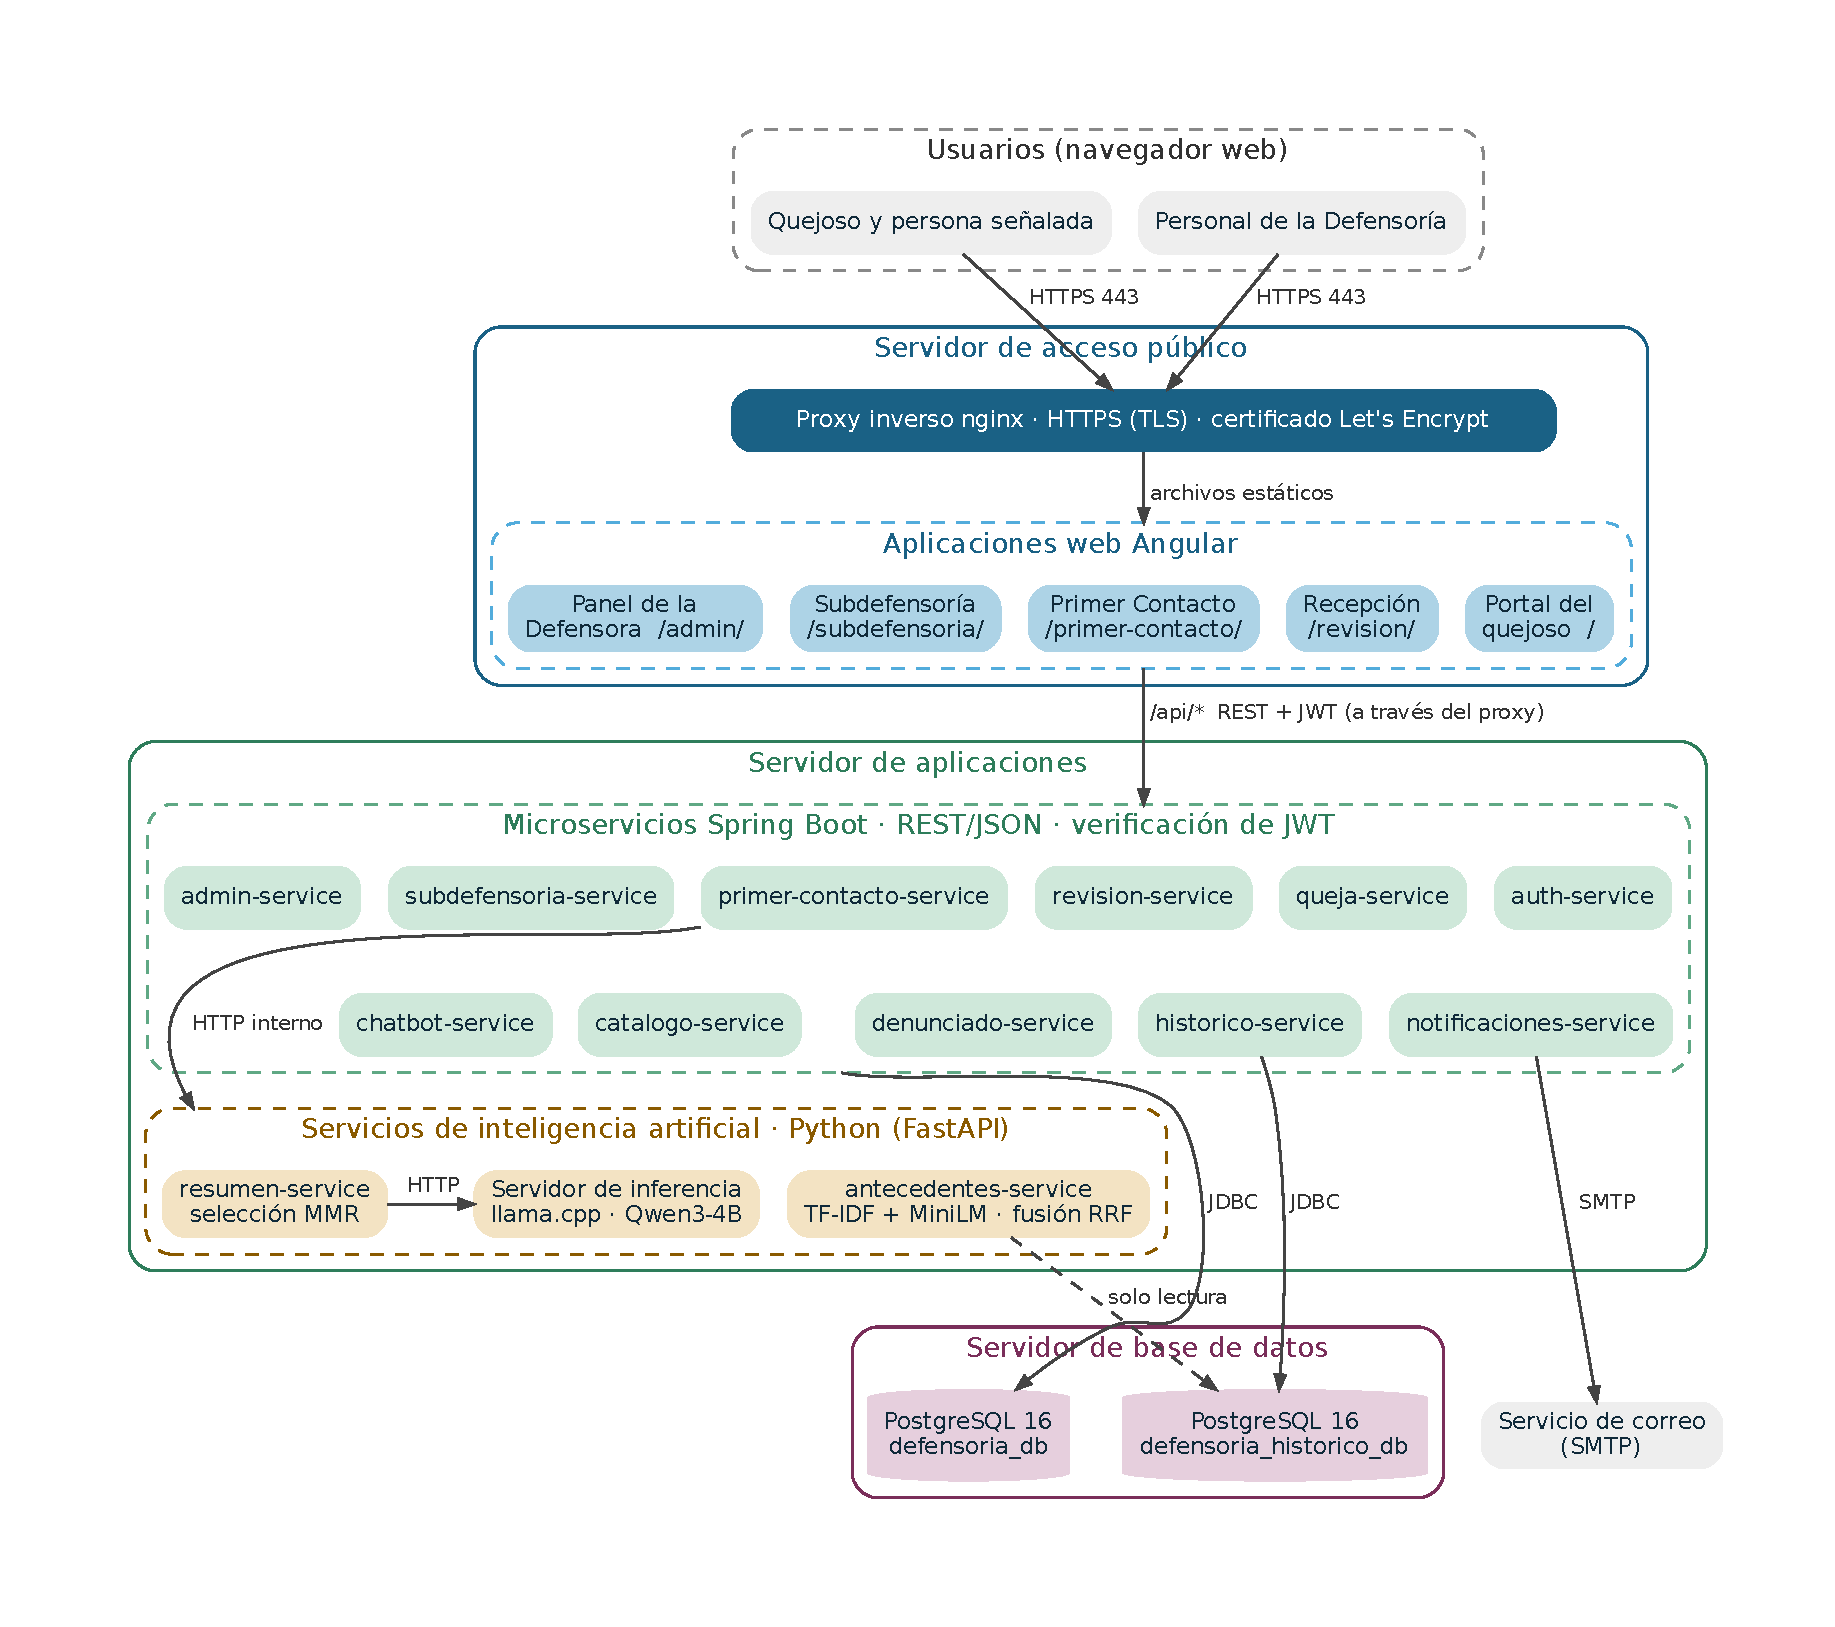
\includegraphics[width=\textwidth]{images/arquitectura.pdf}
	\caption{Arquitectura de la plataforma}
	\label{fig:arquitectura}
\end{figure}

\textbf{Servidor de acceso público.} Es el único expuesto a Internet. Un proxy inverso nginx recibe todas las peticiones por HTTPS, con un certificado de Let's Encrypt, y sirve las cinco aplicaciones web desarrolladas con Angular: el portal del quejoso y los paneles de Recepción, Primer Contacto, Subdefensoría y la Defensora, cada uno publicado en su propia ruta. Las peticiones a la interfaz de programación (\texttt{/api/*}) se reenvían al microservicio correspondiente. Como las aplicaciones y la interfaz de programación se publican bajo el mismo dominio, el navegador las trata como un mismo origen, lo que simplifica la seguridad del lado del cliente.

\textbf{Servidor de aplicaciones.} Aloja once microservicios desarrollados con Spring Boot y tres servicios de inteligencia artificial desarrollados en Python. Cada microservicio atiende un área del procedimiento y se comunica mediante peticiones REST con intercambio de datos en formato JSON. La Tabla~\ref{tab:microservicios} resume su responsabilidad. Los servicios de inteligencia artificial solo son accesibles desde la red interna: el microservicio de Primer Contacto les solicita los antecedentes y los resúmenes, y el servicio de resúmenes, a su vez, consulta al servidor de inferencia que ejecuta el modelo Qwen3 mediante llama.cpp.

\textbf{Servidor de base de datos.} Contiene dos bases de datos PostgreSQL 16: \texttt{defensoria\_db}, con la información operativa de la plataforma, y \texttt{defensoria\_historico\_db}, con las quejas históricas de la Defensoría. Sus puertos solo aceptan conexiones del servidor de aplicaciones.

\rowcolors{2}{rowblue}{white}
\small
\renewcommand{\arraystretch}{1.2}
\setlength{\tabcolsep}{4pt}
\begin{longtable}{|L{4.6cm}|L{11.0cm}|}
	\hiderowcolors\caption{Microservicios y servicios de la plataforma}
	\label{tab:microservicios} \\ \showrowcolors
	\hline
	\rowcolor{headerblue}
	\headercell{Servicio} & \headercell{Responsabilidad} \\
	\hline
	\endfirsthead
	\hline
	\rowcolor{headerblue}
	\headercell{Servicio} & \headercell{Responsabilidad} \\
	\hline
	\endhead
	\texttt{auth-service} & Sesión del quejoso: activación de la cuenta, inicio de sesión, recuperación de contraseña y perfil. Emite los tokens de los quejosos. \\ \hline
	\texttt{queja-service} & Registro de quejas, con o sin cuenta; consulta y edición de las quejas propias, evidencias y respuesta a acuerdos de conciliación. \\ \hline
	\texttt{revision-service} & Bandeja de Recepción: validación, rechazo, turnado, registro manual, historial exportable y emisión de acuerdos. \\ \hline
	\texttt{primer-contacto-service} & Expedientes de análisis, citas, oficios, dictámenes, remisiones y solicitudes a la persona señalada; integra los servicios de antecedentes y de resúmenes. \\ \hline
	\texttt{subdefensoria-service} & Expedientes de investigación, oficios de solicitud de información, control de plazos, recordatorios y acuerdos de conclusión. \\ \hline
	\texttt{denunciado-service} & Registro de la versión de los hechos de la persona señalada y de sus evidencias. \\ \hline
	\texttt{admin-service} & Sesión del personal, cuentas y roles, panel de supervisión de la Defensora, plantillas, respaldos y bitácora. Emite los tokens del personal. \\ \hline
	\texttt{notificaciones-service} & Envío de correos electrónicos y centro de notificaciones de cada usuario. \\ \hline
	\texttt{catalogo-service} & Catálogo de dependencias y unidades académicas y de instancias de remisión. \\ \hline
	\texttt{chatbot-service} & Menú de preguntas frecuentes del portal público y su administración. \\ \hline
	\texttt{historico-service} & Consulta de la información histórica de quejas. \\ \hline
	\texttt{antecedentes-service} & Búsqueda híbrida de antecedentes con TF-IDF y MiniLM sobre las quejas vigentes e históricas (solo lectura). \\ \hline
	\texttt{resumen-service} & Selección extractiva de fragmentos mediante MMR y solicitud de la redacción del resumen al modelo generativo. \\ \hline
	Servidor de inferencia & Ejecución del modelo Qwen3-4B mediante llama.cpp. \\ \hline
\end{longtable}
\normalsize
\setlength{\tabcolsep}{6pt}
\renewcommand{\arraystretch}{1}

\textbf{Seguridad.} La autenticación se basa en tokens JWT firmados. El servicio de autenticación emite los tokens de los quejosos y el de administración los del personal; el resto de los microservicios únicamente los verifican y aplican la autorización según el rol del usuario en cada operación. Las contraseñas se almacenan cifradas mediante una función de resumen. En la red, cada servidor solo acepta conexiones del servidor que le antecede: el de aplicaciones, del de acceso público, y el de base de datos, del de aplicaciones.

\textbf{Comunicación entre servicios.} La comunicación es síncrona sobre HTTP. Además de las peticiones que llegan a través del proxy, existen llamadas internas entre servicios: Primer Contacto envía a Subdefensoría los expedientes dictaminados como procedentes y varios servicios solicitan al servicio de notificaciones el envío de correos. Una falla en un servicio auxiliar, como el de notificaciones o los de inteligencia artificial, no impide que la operación principal se complete (requerimientos RNF-Q04 y RNF-G02).

\textbf{Despliegue.} Todos los componentes se ejecutan en contenedores administrados con Podman, lo que permite actualizar cada servicio de manera independiente.

\section{Diseño de la base de datos}
\label{sec:bd}
La información operativa de la plataforma se almacena en la base de datos \texttt{defensoria\_db}, administrada con PostgreSQL 16. El esquema consta de 29 tablas organizadas en cinco módulos que siguen las etapas del procedimiento: el núcleo de quejas, Primer Contacto, la respuesta de la persona señalada, Subdefensoría, y la administración y los catálogos.

Las tablas se crean a partir de las entidades que declara cada microservicio, de modo que el esquema corresponde directamente al código de la plataforma. Cada tabla tiene un microservicio responsable de su escritura. Dentro de un mismo servicio, las relaciones se declaran como llaves foráneas; entre servicios distintos, en cambio, se emplean \emph{referencias lógicas}: el registro hijo guarda el folio o el identificador del registro padre y la integridad se verifica en la lógica del servicio. Esta decisión mantiene independientes a los microservicios, a cambio de que la base de datos no impida por sí sola una referencia inválida entre módulos.

La Figura~\ref{fig:er_general} presenta el diagrama entidad-relación de la base de datos. Para que el esquema completo pueda leerse en una sola página, presentada en orientación horizontal, de cada tabla se muestran sus atributos clave: la llave primaria, las llaves foráneas, las referencias lógicas y los atributos referenciados por otras tablas, con su tipo de dato. Las tablas se distinguen por color según su módulo. Los atributos restantes de cada tabla y las relaciones de menor nivel ---como la referencia de cada cita, nota o dictamen al analista que la registró, o la cita reprogramada a partir de otra--- se presentan en los diagramas por módulo del Anexo~\ref{anx:base_datos}.

\begin{sidewaysfigure}
	\centering
	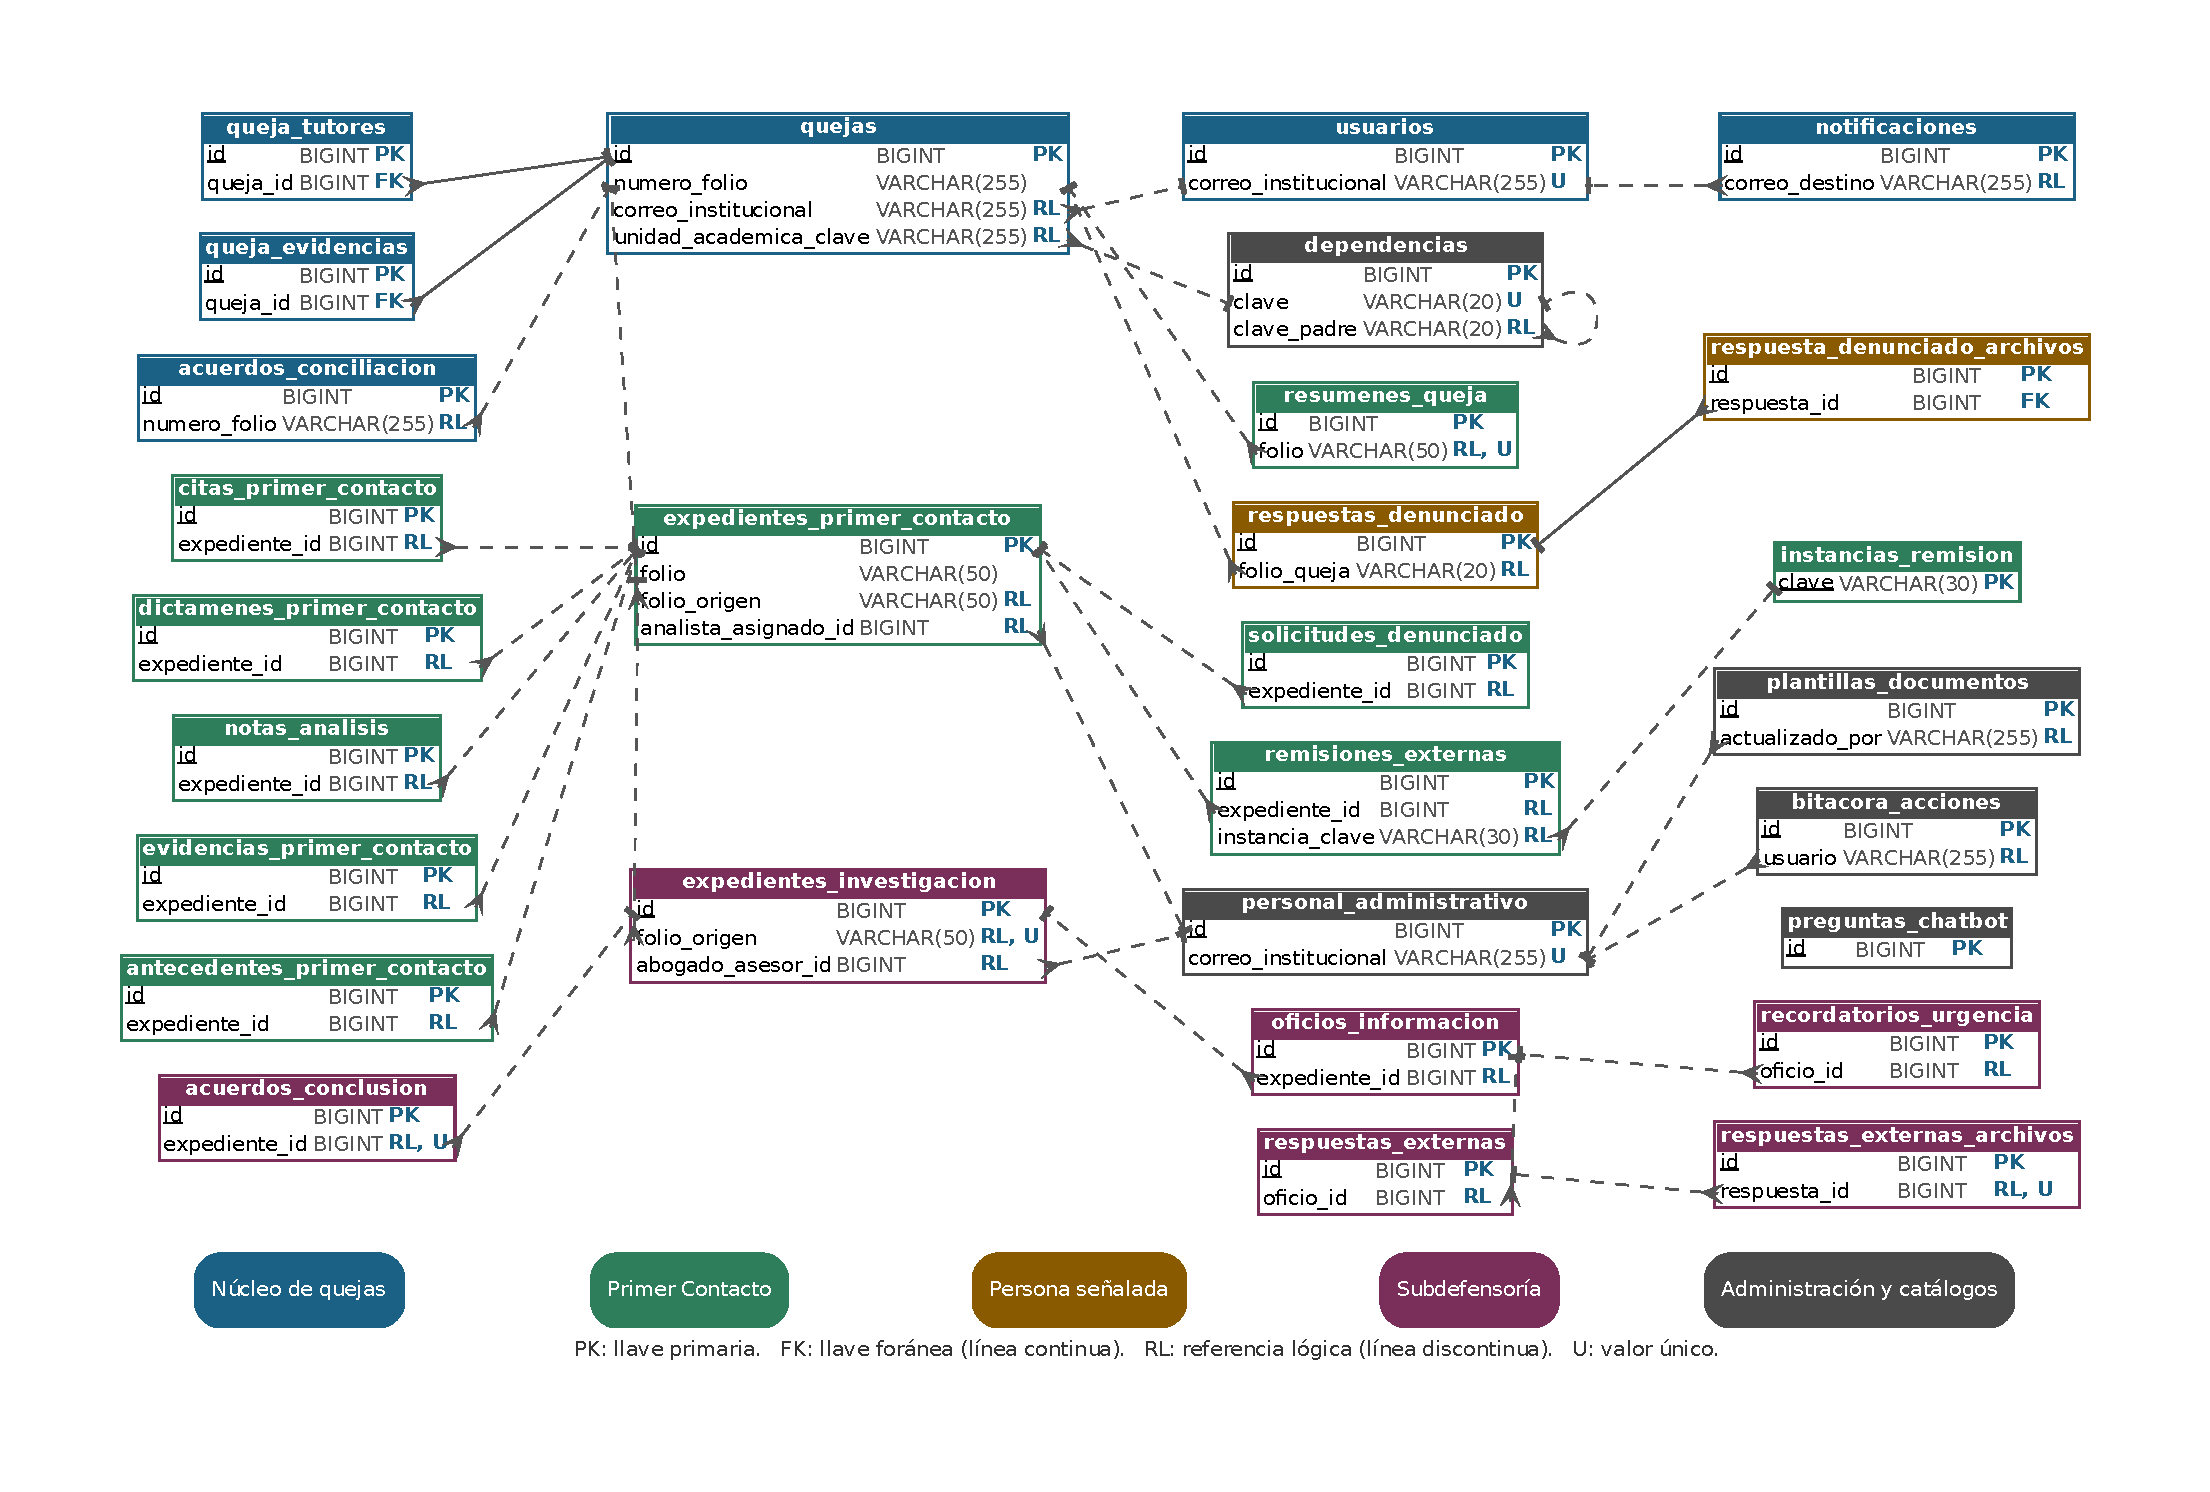
\includegraphics[width=23cm,height=14.6cm,keepaspectratio]{images/er_general.pdf}
	\caption{Diagrama entidad-relación de la base de datos (atributos clave)}
	\label{fig:er_general}
\end{sidewaysfigure}

Algunas tablas se relacionan con el resto del esquema mediante el correo electrónico y no mediante un identificador: \texttt{notificaciones} guarda el correo del destinatario, y \texttt{bitacora\_acciones} y \texttt{plantillas\_documentos} guardan el correo institucional de la persona del personal que realizó la acción o la actualización. La tabla \texttt{dependencias} se relaciona consigo misma para representar la jerarquía de dependencias del Instituto. Por último, \texttt{preguntas\_chatbot} es independiente: almacena el contenido del menú de ayuda del portal público y no depende de ningún otro registro.

El expediente de una queja recorre tres tablas principales, una por cada etapa del procedimiento. La tabla \texttt{quejas} conserva la queja tal como la presentó el quejoso y su paso por Recepción; cuando Recepción la turna, se crea un registro en \texttt{expedientes\_primer\_contacto}, que guarda el folio de la queja original; y cuando Primer Contacto la dictamina como procedente, se crea un registro en \texttt{expedientes\_investigacion}, que guarda el folio de Primer Contacto. Las demás tablas de cada módulo ---citas, dictámenes, oficios, recordatorios, acuerdos--- dependen de alguno de estos tres expedientes. Por esta razón, a continuación se presenta el diccionario de datos de estas tres tablas. En el diccionario se emplea la siguiente notación para la columna \emph{Clave}: PK, llave primaria; FK, llave foránea; RL, referencia lógica; y U, restricción de unicidad.

\subsection{Tablas principales}

\rowcolors{2}{rowblue}{white}
\footnotesize
\renewcommand{\arraystretch}{1.15}
\setlength{\tabcolsep}{4pt}
\begin{longtable}{|L{3.9cm}|L{2.4cm}|L{0.9cm}|L{1.2cm}|L{6.6cm}|}
	\hiderowcolors\caption{Diccionario de datos de la tabla \texttt{quejas}}
	\label{tab:cap3_dic_quejas} \\ \showrowcolors
	\hline
	\rowcolor{headerblue}
	\headercell{Columna} & \headercell{Tipo} & \headercell{Nulo} & \headercell{Clave} & \headercell{Descripción} \\
	\hline
	\endfirsthead
	\hline
	\rowcolor{headerblue}
	\headercell{Columna} & \headercell{Tipo} & \headercell{Nulo} & \headercell{Clave} & \headercell{Descripción} \\
	\hline
	\endhead
		\texttt{id} & BIGINT & No & PK & Identificador único del registro, generado automáticamente. \\ \hline
		\texttt{numero\_\allowbreak{}folio} & VARCHAR(255) & No &  & Folio de seguimiento que se entrega al quejoso. \\ \hline
		\texttt{correo\_\allowbreak{}institucional} & VARCHAR(255) & No & RL & Correo del quejoso; junto con el folio permite consultar la queja y activar la cuenta. \\ \hline
		\texttt{estatus} & VARCHAR(255) & Sí &  & Estatus de la queja (RECIBIDA, EN\_VALIDACION, RECHAZADA, TURNADA, entre otros). \\ \hline
		\texttt{motivo} & VARCHAR(255) & No &  & Motivo de la queja. \\ \hline
		\texttt{descripcion} & TEXT & Sí &  & Narrativa de los hechos redactada por el quejoso. \\ \hline
		\texttt{unidad\_\allowbreak{}academica\_\allowbreak{}clave} & VARCHAR(255) & Sí & RL & Clave de la unidad académica involucrada, tomada del catálogo. \\ \hline
		\texttt{fecha\_\allowbreak{}creacion} & TIMESTAMP & Sí &  & Fecha y hora en que se registró la queja. \\ \hline
		\texttt{fecha\_\allowbreak{}hechos} & DATE & Sí &  & Fecha en que ocurrieron los hechos. \\ \hline
		\texttt{nombre\_\allowbreak{}quejoso} & VARCHAR(255) & Sí &  & Nombre del quejoso. \\ \hline
		\texttt{apellido1\_\allowbreak{}quejoso} & VARCHAR(255) & Sí &  & Primer apellido del quejoso. \\ \hline
		\texttt{apellido2\_\allowbreak{}quejoso} & VARCHAR(255) & Sí &  & Segundo apellido del quejoso. \\ \hline
		\texttt{numero\_\allowbreak{}identificacion\_\allowbreak{}quejoso} & VARCHAR(255) & Sí &  & Número de boleta o de empleado del quejoso. \\ \hline
		\texttt{tipo\_\allowbreak{}identificacion\_\allowbreak{}quejoso} & VARCHAR(255) & Sí &  & Tipo de identificación del quejoso. \\ \hline
		\texttt{fecha\_\allowbreak{}nacimiento\_\allowbreak{}quejoso} & DATE & Sí &  & Fecha de nacimiento del quejoso, usada para identificar a menores de edad. \\ \hline
		\texttt{nombre\_\allowbreak{}denunciado} & VARCHAR(255) & Sí &  & Nombre de la persona señalada. \\ \hline
		\texttt{apellido1\_\allowbreak{}denunciado} & VARCHAR(255) & Sí &  & Primer apellido de la persona señalada. \\ \hline
		\texttt{apellido2\_\allowbreak{}denunciado} & VARCHAR(255) & Sí &  & Segundo apellido de la persona señalada. \\ \hline
		\texttt{folio\_\allowbreak{}primer\_\allowbreak{}contacto} & VARCHAR(255) & Sí &  & Folio asignado en Primer Contacto. \\ \hline
		\texttt{ruta\_\allowbreak{}evidencia} & VARCHAR(255) & Sí &  & Ruta de la evidencia principal de la queja. \\ \hline
		\texttt{aviso\_\allowbreak{}privacidad\_\allowbreak{}aceptado} & BOOLEAN & Sí &  & Indica si se aceptó el aviso de privacidad. \\ \hline
		\texttt{aviso\_\allowbreak{}privacidad\_\allowbreak{}fecha} & TIMESTAMP & Sí &  & Fecha y hora de aceptación del aviso de privacidad. \\ \hline
		\texttt{aviso\_\allowbreak{}privacidad\_\allowbreak{}version} & VARCHAR(255) & Sí &  & Versión del aviso de privacidad aceptada. \\ \hline
		\texttt{origen\_\allowbreak{}registro} & VARCHAR(255) & Sí &  & Punto de acceso por el que ingresó la queja (público, autenticado o manual). \\ \hline
		\texttt{motivo\_\allowbreak{}rechazo} & TEXT & Sí &  & Motivos y observaciones del rechazo. \\ \hline
		\texttt{validado\_\allowbreak{}por} & VARCHAR(255) & Sí & RL & Correo de la persona de Recepción que validó la queja. \\ \hline
		\texttt{area\_\allowbreak{}turnada} & VARCHAR(255) & Sí &  & Área a la que Recepción turnó la queja. \\ \hline
		\texttt{fecha\_\allowbreak{}turnado} & TIMESTAMP & Sí &  & Fecha y hora del turnado. \\ \hline
		\texttt{tutor\_\allowbreak{}id} & BIGINT & Sí & FK & Tutor asociado a la queja, cuando el quejoso es menor de edad. \\ \hline
		\texttt{defensor\_\allowbreak{}asignado} & VARCHAR(255) & Sí &  & Defensor o analista al que se asignó la queja al turnarla. \\ \hline
		\texttt{comentarios\_\allowbreak{}recepcion} & TEXT & Sí &  & Comentarios de Recepción al turnar la queja. \\ \hline
		\texttt{fecha\_\allowbreak{}validacion} & TIMESTAMP & Sí &  & Fecha y hora de la validación por Recepción. \\ \hline
		\texttt{revisando\_\allowbreak{}por} & VARCHAR(255) & Sí &  & Correo de la persona de Recepción que tiene tomada la queja. \\ \hline
		\texttt{revisando\_\allowbreak{}por\_\allowbreak{}nombre} & VARCHAR(255) & Sí &  & Nombre de la persona de Recepción que tiene tomada la queja. \\ \hline
		\texttt{fecha\_\allowbreak{}inicio\_\allowbreak{}revision} & TIMESTAMP & Sí &  & Fecha y hora en que Recepción tomó la queja para revisarla. \\ \hline
		\texttt{estatus\_\allowbreak{}previo\_\allowbreak{}revision} & VARCHAR(255) & Sí &  & Estatus que tenía la queja antes de que Recepción la tomara. \\ \hline
		\texttt{numero\_\allowbreak{}oficio} & VARCHAR(255) & Sí &  & Número del oficio. \\ \hline
		\texttt{fecha\_\allowbreak{}recepcion\_\allowbreak{}fisica} & DATE & Sí &  & Fecha de recepción del documento físico. \\ \hline
		\texttt{tipo\_\allowbreak{}documento\_\allowbreak{}fisico} & VARCHAR(255) & Sí &  & Tipo del documento físico recibido. \\ \hline
		\texttt{ubicacion\_\allowbreak{}fisica\_\allowbreak{}expediente} & VARCHAR(255) & Sí &  & Ubicación física del expediente en papel. \\ \hline
		\texttt{tipo\_\allowbreak{}usuario\_\allowbreak{}manual} & VARCHAR(255) & Sí &  & Tipo de usuario capturado en el registro manual. \\ \hline
		\texttt{telefono\_\allowbreak{}contacto} & VARCHAR(255) & Sí &  & Teléfono de contacto del quejoso. \\ \hline
\end{longtable}
\normalsize
\setlength{\tabcolsep}{6pt}
\renewcommand{\arraystretch}{1}

\rowcolors{2}{rowblue}{white}
\footnotesize
\renewcommand{\arraystretch}{1.15}
\setlength{\tabcolsep}{4pt}
\begin{longtable}{|L{3.9cm}|L{2.4cm}|L{0.9cm}|L{1.2cm}|L{6.6cm}|}
	\hiderowcolors\caption{Diccionario de datos de la tabla \texttt{expedientes\_primer\_contacto}}
	\label{tab:cap3_dic_expedientes_primer_contacto} \\ \showrowcolors
	\hline
	\rowcolor{headerblue}
	\headercell{Columna} & \headercell{Tipo} & \headercell{Nulo} & \headercell{Clave} & \headercell{Descripción} \\
	\hline
	\endfirsthead
	\hline
	\rowcolor{headerblue}
	\headercell{Columna} & \headercell{Tipo} & \headercell{Nulo} & \headercell{Clave} & \headercell{Descripción} \\
	\hline
	\endhead
		\texttt{id} & BIGINT & No & PK & Identificador único del registro, generado automáticamente. \\ \hline
		\texttt{folio} & VARCHAR(50) & No &  & Folio del expediente en Primer Contacto. \\ \hline
		\texttt{folio\_\allowbreak{}origen} & VARCHAR(50) & No & RL & Folio de la queja original. \\ \hline
		\texttt{tema} & VARCHAR(200) & Sí &  & Tema o motivo de la queja. \\ \hline
		\texttt{descripcion\_\allowbreak{}hechos} & TEXT & Sí &  & Narrativa de los hechos copiada de la queja. \\ \hline
		\texttt{fecha\_\allowbreak{}recepcion\_\allowbreak{}origen} & VARCHAR(50) & Sí &  & Fecha de recepción de la queja original. \\ \hline
		\texttt{prioridad} & VARCHAR(30) & Sí &  & Prioridad del expediente (baja, media, alta o urgente). \\ \hline
		\texttt{quejoso\_\allowbreak{}nombre} & VARCHAR(200) & Sí &  & Nombre del quejoso. \\ \hline
		\texttt{quejoso\_\allowbreak{}correo} & VARCHAR(150) & Sí &  & Correo electrónico del quejoso. \\ \hline
		\texttt{unidad\_\allowbreak{}academica} & VARCHAR(200) & Sí &  & Unidad académica relacionada. \\ \hline
		\texttt{estatus} & VARCHAR(40) & No &  & Estatus del análisis (TURNADA, EN\_ANALISIS, PROCEDENTE, IMPROCEDENTE, REMITIDA, entre otros). \\ \hline
		\texttt{fecha\_\allowbreak{}inicio\_\allowbreak{}analisis} & TIMESTAMP & Sí &  & Fecha y hora en que inició el análisis. \\ \hline
		\texttt{analista\_\allowbreak{}analisis\_\allowbreak{}id} & BIGINT & Sí &  & Identificador del analista que inició el análisis. \\ \hline
		\texttt{analista\_\allowbreak{}analisis\_\allowbreak{}nombre} & VARCHAR(150) & Sí &  & Nombre del analista que inició el análisis. \\ \hline
		\texttt{analista\_\allowbreak{}asignado\_\allowbreak{}id} & BIGINT & Sí & RL & Identificador del analista al que Recepción turnó el expediente. \\ \hline
		\texttt{analista\_\allowbreak{}asignado\_\allowbreak{}nombre} & VARCHAR(150) & Sí &  & Nombre del analista asignado. \\ \hline
		\texttt{fecha\_\allowbreak{}creacion} & TIMESTAMP & No &  & Fecha y hora de creación del registro. \\ \hline
		\texttt{fecha\_\allowbreak{}actualizacion} & TIMESTAMP & Sí &  & Fecha y hora de la última actualización. \\ \hline
		\texttt{folio\_\allowbreak{}subdefensoria} & VARCHAR(50) & Sí & U & Folio del expediente de investigación en Subdefensoría. \\ \hline
		\texttt{quejoso\_\allowbreak{}id} & BIGINT & Sí &  & Identificador de la cuenta del quejoso, si existe. \\ \hline
		\texttt{quejoso\_\allowbreak{}telefono} & VARCHAR(30) & Sí &  & Teléfono del quejoso. \\ \hline
		\texttt{quejoso\_\allowbreak{}tipo\_\allowbreak{}usuario} & VARCHAR(50) & Sí &  & Tipo de usuario del quejoso (alumno, personal, etc.). \\ \hline
\end{longtable}
\normalsize
\setlength{\tabcolsep}{6pt}
\renewcommand{\arraystretch}{1}

\rowcolors{2}{rowblue}{white}
\footnotesize
\renewcommand{\arraystretch}{1.15}
\setlength{\tabcolsep}{4pt}
\begin{longtable}{|L{3.9cm}|L{2.4cm}|L{0.9cm}|L{1.2cm}|L{6.6cm}|}
	\hiderowcolors\caption{Diccionario de datos de la tabla \texttt{expedientes\_investigacion}}
	\label{tab:cap3_dic_expedientes_investigacion} \\ \showrowcolors
	\hline
	\rowcolor{headerblue}
	\headercell{Columna} & \headercell{Tipo} & \headercell{Nulo} & \headercell{Clave} & \headercell{Descripción} \\
	\hline
	\endfirsthead
	\hline
	\rowcolor{headerblue}
	\headercell{Columna} & \headercell{Tipo} & \headercell{Nulo} & \headercell{Clave} & \headercell{Descripción} \\
	\hline
	\endhead
		\texttt{id} & BIGINT & No & PK & Identificador único del registro, generado automáticamente. \\ \hline
		\texttt{folio} & VARCHAR(50) & No & U & Folio del expediente en Subdefensoría. \\ \hline
		\texttt{folio\_\allowbreak{}origen} & VARCHAR(50) & No & RL, U & Folio del expediente en Primer Contacto. \\ \hline
		\texttt{folio\_\allowbreak{}queja} & VARCHAR(50) & Sí &  & Folio de la queja original. \\ \hline
		\texttt{quejoso\_\allowbreak{}nombre} & VARCHAR(150) & Sí &  & Nombre del quejoso. \\ \hline
		\texttt{quejoso\_\allowbreak{}correo} & VARCHAR(150) & Sí &  & Correo electrónico del quejoso. \\ \hline
		\texttt{unidad\_\allowbreak{}academica} & VARCHAR(100) & Sí &  & Unidad académica relacionada. \\ \hline
		\texttt{asunto} & VARCHAR(200) & Sí &  & Asunto o tema del documento. \\ \hline
		\texttt{descripcion\_\allowbreak{}hechos} & TEXT & Sí &  & Narrativa de los hechos de la queja. \\ \hline
		\texttt{fecha\_\allowbreak{}admision} & DATE & No &  & Fecha en que el expediente se admitió en Subdefensoría. \\ \hline
		\texttt{abogado\_\allowbreak{}asesor\_\allowbreak{}id} & BIGINT & Sí & RL & Identificador del abogado de Subdefensoría asignado (personal administrativo). \\ \hline
		\texttt{abogado\_\allowbreak{}asesor\_\allowbreak{}nombre} & VARCHAR(150) & Sí &  & Nombre del abogado asignado, conservado para consulta. \\ \hline
		\texttt{estatus} & VARCHAR(30) & No &  & Etapa de la investigación (RECIBIDO, EN\_INVESTIGACION, EN\_ESPERA\_OFICIO, CONCLUIDO, entre otras). \\ \hline
		\texttt{observaciones\_\allowbreak{}analista} & TEXT & Sí &  & Observaciones del analista de Primer Contacto al turnar. \\ \hline
		\texttt{prioridad} & VARCHAR(10) & Sí &  & Prioridad del expediente (baja, media, alta o urgente). \\ \hline
		\texttt{fecha\_\allowbreak{}creacion} & TIMESTAMP & No &  & Fecha y hora de creación del registro. \\ \hline
		\texttt{fecha\_\allowbreak{}actualizacion} & TIMESTAMP & Sí &  & Fecha y hora de la última actualización. \\ \hline
\end{longtable}
\normalsize
\setlength{\tabcolsep}{6pt}
\renewcommand{\arraystretch}{1}

\noindent\textbf{Nota:} los diagramas entidad-relación de cada módulo con todas sus columnas y el diccionario de datos completo de las 29 tablas se presentan en el Anexo~\ref{anx:base_datos}.
